\documentclass[aspectratio=169,11pt]{beamer}
\usepackage[bahasa]{babel}
\usepackage[utf8]{inputenc}
\usepackage[T1]{fontenc}
\usepackage{tabularx}
\usepackage{booktabs}
\usepackage{tikz}
\usepackage{graphicx}
\usepackage[most]{tcolorbox}
\usepackage{amsmath}
\usepackage{amssymb}
\usetikzlibrary{positioning, arrows.meta, shapes.geometric, shapes.misc, backgrounds, fit, calc, shadows}

% Font profesional: Source Sans Pro (fallback ke helvet jika tidak tersedia)
\IfFileExists{sourcesanspro.sty}{%
    \usepackage[default]{sourcesanspro}%
}{%
    \usepackage[scaled]{helvet}%
    \renewcommand{\familydefault}{\sfdefault}%
}
\usepackage{sfmath}
\usefonttheme{professionalfonts}

% Warna Korporat PLN + Premium Accents
\definecolor{plnblue}{RGB}{0,75,135}
\definecolor{plnorange}{RGB}{255,107,53}
\definecolor{plncyan}{RGB}{0,163,224}
\definecolor{plngreen}{RGB}{0,150,136}
\definecolor{lightgrey}{RGB}{248,249,250}
\definecolor{darkgrey}{RGB}{50,50,50}

% Warna Evolusi Paradigma (Modern Slate/Blue)
\definecolor{TitleDark}{HTML}{0F172A}
\definecolor{TitleSub}{HTML}{64748B}
\definecolor{PilarLeft}{HTML}{64748B}
\definecolor{PilarRight}{HTML}{0284C7}
\definecolor{DimCenter}{HTML}{475569}
\definecolor{NodeLeftBg}{HTML}{F1F5F9}
\definecolor{NodeLeftBorder}{HTML}{94A3B8}
\definecolor{NodeRightBg}{HTML}{E0F2FE}
\definecolor{FoundBg1}{HTML}{0F172A}
\definecolor{FoundTitle}{HTML}{38BDF8}
\definecolor{FoundHighlight}{HTML}{FDE047}
\definecolor{CircuitColor}{HTML}{38BDF8}

% TikZ BPMN Styles
\tikzset{
    startstyle/.style={circle, draw=red!70!black, fill=red!15, minimum size=0.9cm, align=center, font=\tiny\bfseries, line width=1pt},
    endstyle/.style={circle, draw=red!70!black, fill=red!25, minimum size=0.9cm, align=center, font=\tiny\bfseries, line width=1.5pt},
    startstyle_tobe/.style={circle, draw=green!60!black, fill=green!15, minimum size=0.9cm, align=center, font=\tiny\bfseries, line width=1pt},
    endstyle_tobe/.style={circle, draw=plnblue!80!black, fill=plnblue!25, minimum size=0.9cm, align=center, font=\tiny\bfseries, line width=1.5pt},
    manual/.style={rectangle, rounded corners=2pt, draw=gray!70, fill=gray!8, text width=2.4cm, minimum height=1.2cm, align=center, font=\tiny, line width=0.6pt},
    waiting/.style={rectangle, rounded corners=2pt, draw=red!50, fill=red!5, text width=2.4cm, minimum height=1.2cm, align=center, font=\tiny\itshape, line width=0.6pt},
    autostep/.style={rectangle, rounded corners=2pt, draw=plnblue!80, fill=plnblue!12, text width=2.4cm, minimum height=1.2cm, align=center, font=\tiny\bfseries, line width=0.6pt},
    humanstep/.style={rectangle, rounded corners=2pt, draw=plnorange, fill=plnorange!10, text width=2.4cm, minimum height=1.2cm, align=center, font=\tiny, line width=0.6pt},
    gateway/.style={diamond, draw=gray!70, fill=yellow!8, minimum width=1.1cm, minimum height=1.1cm, align=center, font=\tiny\bfseries, inner sep=1pt, aspect=1},
    gateway_tobe/.style={diamond, draw=plnorange!80, fill=plnorange!8, minimum width=1.1cm, minimum height=1.1cm, align=center, font=\tiny\bfseries, inner sep=1pt, aspect=1},
    arr/.style={-{Stealth[length=5pt]}, thick, color=gray!60},
    arr_tobe/.style={-{Stealth[length=5pt]}, thick, color=plnblue!70},
    arrok/.style={-{Stealth[length=5pt]}, thick, color=green!60!black},
    arrno/.style={-{Stealth[length=5pt]}, thick, color=red!50, dashed},
    apimsg/.style={-{Stealth[length=6pt]}, dashed, thick, color=gray!80!black},
    timelbl/.style={font=\tiny\bfseries, text=red!60!black},
    timelbl_tobe/.style={font=\tiny\bfseries, text=green!50!black},
    lanelab/.style={font=\tiny\bfseries, text=gray!70!black, rotate=90},
    % New Styles for Metadata Journey
    meta/.style={circle, fill=#1, text=white, font=\fontsize{3}{4}\selectfont\bfseries, inner sep=1pt, minimum size=0.9cm, align=center},
    docstyle/.style={rectangle, fill=white, draw=plnblue, line width=1.5pt, minimum width=2.2cm, minimum height=3.2cm, drop shadow}
}


% Konfigurasi Tema Beamer Premium
\mode<presentation>{
    \usetheme{Madrid}
    \usecolortheme[named=plnblue]{structure}
    \setbeamercolor{palette primary}{bg=plnblue,fg=white}
    \setbeamercolor{palette secondary}{bg=plnorange,fg=white}
    \setbeamercolor{title}{bg=plnblue,fg=white}
    \setbeamercolor{frametitle}{bg=,fg=plnblue}
    \setbeamerfont{frametitle}{series=\bfseries, size=\large}
    \setbeamercolor{background canvas}{bg=white}
    \setbeamertemplate{navigation symbols}{}
    \setbeamertemplate{items}[circle]
    
    % Background default untuk slide isi (content)
    \usebackgroundtemplate{
\includegraphics[width=\paperwidth,height=\paperheight]{assets/content.png}}
    
    % Footer minimalis: hanya nomor halaman kanan bawah tanpa background
    \setbeamertemplate{footline}{%
        \hfill\textcolor{plnblue}{\insertframenumber{} / \inserttotalframenumber}\hspace{1em}\vspace{0.5em}%
    }
    
    % Frametitle center alignment tanpa background, posisi lebih turun
    \setbeamertemplate{frametitle}{%
        \vspace{0.3cm}%
        \centering%
        \usebeamerfont{frametitle}\usebeamercolor[fg]{frametitle}\insertframetitle\par%
        \vspace{0.05cm}%
    }
}

% Custom Boxes
\newtcolorbox{premiumbox}[1][]{%
  colback=plnblue!5!white, colframe=plnblue, fonttitle=\bfseries\small,
  sharp corners, boxrule=1pt, left=4pt, right=4pt, top=4pt, bottom=4pt,
  title={#1}, before skip=4pt, after skip=10pt, breakable
}

\newtcolorbox{orangebox}[1][]{%
  colback=plnorange!5!white, colframe=plnorange, fonttitle=\bfseries\small,
  sharp corners, boxrule=1pt, left=4pt, right=4pt, top=4pt, bottom=4pt,
  title={#1}, before skip=4pt, after skip=10pt, breakable
}

\newtcolorbox{greenbox}[1][]{%
  colback=plngreen!5!white, colframe=plngreen, fonttitle=\bfseries\small,
  sharp corners, boxrule=1pt, left=4pt, right=4pt, top=4pt, bottom=4pt,
  title={#1}, before skip=4pt, after skip=10pt, breakable
}

\title{Optimalisasi Prosedur \& Alur Kerja Terintegrasi}
\subtitle{Modul Pelatihan Level 4 (Mastery) -- Transformasi Tata Kelola Kearsipan\\ \textbf{PT PLN (Persero)}}
\author{}
\institute[PLN]{}
\date{}

% Makro untuk Icon Sederhana
\newcommand{\stepicon}[2]{
    \begin{tikzpicture}
        \node[circle, fill=#1, text=white, minimum size=0.6cm, inner sep=0, font=\tiny\bfseries] {#2};
    \end{tikzpicture}
}

% Section divider dengan background section.png
\AtBeginSection[]{
  {
    \usebackgroundtemplate{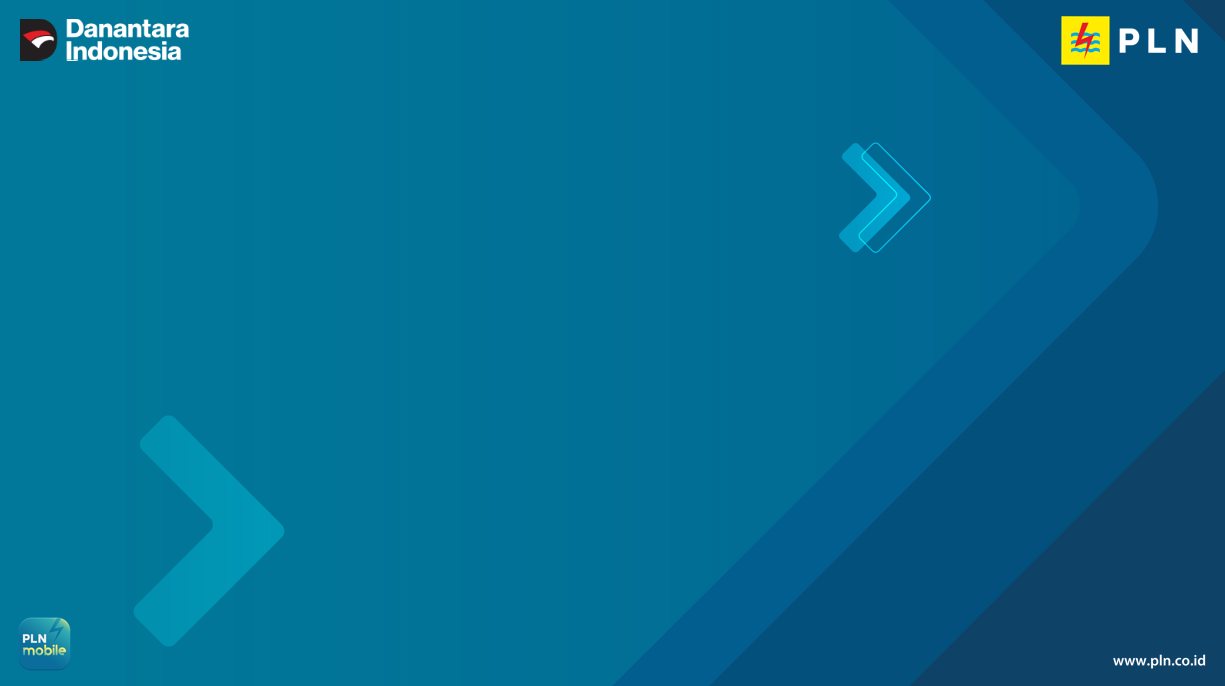
\includegraphics[width=\paperwidth,height=\paperheight]{assets/section.png}}
    \begin{frame}[plain]
      \vfill
      \centering
      {\Huge\bfseries\textcolor{white}{\insertsectionhead}\par}
      \vspace{0.5cm}
      {\large\textcolor{white!80}{Modul 4.3: Optimalisasi Prosedur \& Alur Kerja Terintegrasi}\par}
      \vfill
    \end{frame}
  }
}

\begin{document}

% ================================================================
%  BAGIAN PEMBUKA (5 Menit)
% ================================================================

% SLIDE 1: TITLE PAGE
{
\usebackgroundtemplate{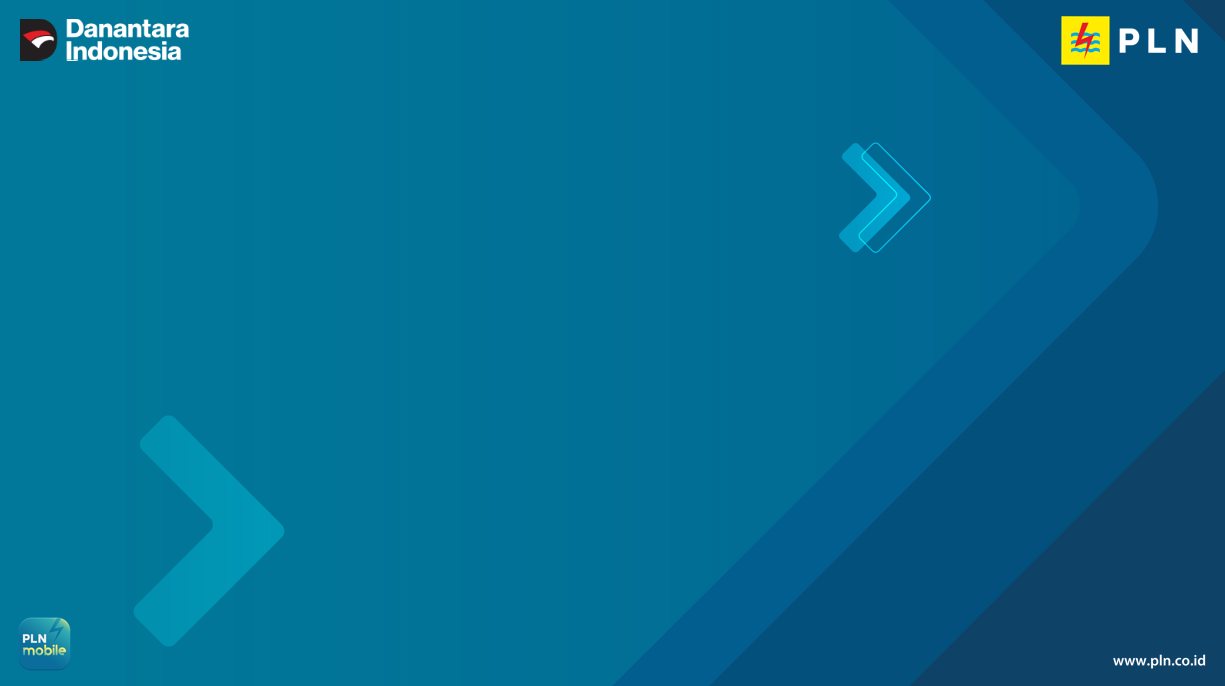
\includegraphics[width=\paperwidth,height=\paperheight]{assets/section.png}}
\setbeamercolor{title}{fg=white}
\setbeamercolor{author}{fg=white}
\setbeamercolor{institute}{fg=white}
\setbeamercolor{date}{fg=white}
\beamertemplatenavigationsymbolsempty
\begin{frame}[plain]
    \titlepage
\end{frame}
}

% SLIDE 2: SASARAN & PRASYARAT PESERTA
\begin{frame}{Sasaran \& Prasyarat Peserta}
    \vspace{0.2cm}
    \begin{columns}[T]
        \column{0.48\textwidth}
        \begin{premiumbox}[Target Peserta]
            \small
            Modul ini ditujukan secara khusus bagi:
            \begin{itemize}
                \item \textbf{Manajemen Atas (MA)} PT PLN (Persero).
                \item Pemilik Proses Bisnis (\textit{Business Process Owner}).
                \item Pengambil Kebijakan Tata Kelola Kearsipan \& Transformasi Digital.
            \end{itemize}
        \end{premiumbox}
        
        \column{0.48\textwidth}
        \begin{orangebox}[Prasyarat Peserta]
            \scriptsize
            Untuk efektivitas pembelajaran, peserta diharapkan:
            \begin{itemize}
                \item Memahami dasar kearsipan (Level 2 atau pengalaman $\ge$ 2 tahun).
                \item Telah mengikuti \textbf{Modul 4.1} (Analisis Sistem) \& \textbf{4.2} (Arsitektur Terintegrasi).
                \item Membawa 1 contoh prosedur riil unit kerja untuk studi kasus workshop.
                \item Meninjau \textit{World Bank RM Roadmap} \& Perka ANRI No. 6/2021.
            \end{itemize}
        \end{orangebox}
    \end{columns}
\end{frame}

% SLIDE 3: TUJUAN PEMBELAJARAN
\begin{frame}{Tujuan Pembelajaran \& Hasil Belajar}
    \vspace{0.2cm}
    \begin{premiumbox}[Kompetensi Akhir Modul Level 4 (Mastery)]
        \small
        Setelah menyelesaikan pelatihan ini, peserta ditargetkan mampu:
    \end{premiumbox}
    \vspace{0.3cm}
    \begin{columns}[T]
        \column{0.45\textwidth}
        \stepicon{plnblue}{1} \textbf{Mengevaluasi Prosedur}\\
        \vspace{0.1cm}
        \small
        Mengevaluasi prosedur kearsipan yang ada (\textit{as-is}) dan mengidentifikasi area yang dapat dioptimalkan melalui integrasi.
        \vspace{0.3cm}
        
        \stepicon{plncyan}{2} \textbf{Merancang Alur Kerja}\\
        \vspace{0.1cm}
        \small
        Merancang alur kerja baru yang terintegrasi (To-Be), termasuk mekanisme penciptaan arsip otomatis dari aplikasi korporat.
        
        \column{0.48\textwidth}
        \stepicon{plnorange}{3} \textbf{Merumuskan SOP Digital}\\
        \vspace{0.1cm}
        \small
        Merumuskan Standard Operating Procedure (SOP) digital yang mengintegrasikan peran manusia, \textit{audit trail} sistem, dan keamanan.
        \vspace{0.3cm}
        
        \stepicon{plngreen}{4} \textbf{Menganalisis Efektivitas}\\
        \vspace{0.1cm}
        \small
        Menganalisis potensi peningkatan layanan dan efisiensi melalui pengukuran indikator kinerja (\textit{KPI}) termonitor.
    \end{columns}
\end{frame}

% SLIDE 4: MANFAAT BAGI PESERTA DIKLAT
\begin{frame}{Manfaat bagi Peserta Diklat}
    \vspace{0.2cm}
    \begin{columns}[T]
        \column{0.48\textwidth}
        \begin{premiumbox}[Manfaat Profesional]
            \small
            \begin{itemize}
                \item \textbf{Dokumen Siap Implementasi:} Peserta membawa 4 portofolio kerja (Matriks Optimasi, BPMN To-Be, Draft SOP Digital, KPI Tracker) yang dapat langsung diusulkan sebagai \textit{pilot project}.
                \item \textbf{Penguasaan Standar Internasional:} Memahami penerapan ISO 15489 \& PARBICA Toolkit dalam konteks operasional PLN.
                \item \textbf{Kapabilitas Evaluasi:} Mampu mengidentifikasi inefisiensi prosedur secara mandiri.
            \end{itemize}
        \end{premiumbox}
        
        \column{0.48\textwidth}
        \begin{orangebox}[Manfaat bagi Unit Kerja]
            \small
            \begin{itemize}
                \item \textbf{Efisiensi Operasional:} Potensi percepatan siklus kearsipan dari 3--5 hari menjadi $<$24 jam.
                \item \textbf{Mitigasi Risiko Kepatuhan:} Kesiapan audit melalui \textit{audit trail} otomatis dan metadata terstandar.
                \item \textbf{Penghematan Biaya:} Estimasi ROI hingga 550\% melalui eliminasi proses manual dan redundansi data.
            \end{itemize}
        \end{orangebox}
    \end{columns}
\end{frame}

% SLIDE 5: AGENDA PEMBELAJARAN (FIX #9: Alokasi Waktu)
\begin{frame}{Agenda Pembelajaran (Outline Materi)}
    \begin{columns}[T]
        \column{0.31\textwidth}
        \begin{tcolorbox}[colback=plnblue!5!white, colframe=plnblue, fonttitle=\bfseries\footnotesize, sharp corners, boxrule=0.6pt, left=2pt, right=2pt, top=0.5pt, bottom=0.5pt, title={Bagian I:\\Fondasi \& Diagnosa}]
            \makebox[\linewidth][r]{%
                \tcbox[on line, colback=plnblue!15, colframe=plnblue, boxrule=0.5pt, arc=2pt, boxsep=0pt, left=2pt, right=2pt, top=0.5pt, bottom=0.5pt, fontupper=\bfseries\tiny\color{plnblue}]{15 menit}%
            }
            
            \scriptsize
            \stepicon{plnblue}{1} \textbf{Pendahuluan \& Urgensi}\\
            {\tiny Visi Ekosistem Digital \& Biaya Tersembunyi.}\\
            \stepicon{plnblue}{2} \textbf{Landasan Internasional}\\
            {\tiny PARBICA, Continuum, \& ISO 15489.}\\
            \stepicon{plnblue}{3} \textbf{Evaluasi Prosedur Lapangan}\\
            {\tiny Identifikasi Friction \& BPMN As-Is.}
        \end{tcolorbox}
        
        \column{0.31\textwidth}
        \begin{tcolorbox}[colback=plnorange!5!white, colframe=plnorange, fonttitle=\bfseries\footnotesize, sharp corners, boxrule=0.6pt, left=2pt, right=2pt, top=0.5pt, bottom=0.5pt, title={Bagian II:\\Desain \& Implementasi}]
            \makebox[\linewidth][r]{%
                \tcbox[on line, colback=plnorange!15, colframe=plnorange, boxrule=0.5pt, arc=2pt, boxsep=0pt, left=2pt, right=2pt, top=0.5pt, bottom=0.5pt, fontupper=\bfseries\tiny\color{plnorange}]{20 menit}%
            }
            
            \scriptsize
            \stepicon{plnorange}{4} \textbf{Perancangan Alur Terintegrasi}\\
            {\tiny Model To-Be, Pola Otomasi, \& Diskusi BPMN.}\\
            \stepicon{plnorange}{5} \textbf{Penyusunan SOP Digital}\\
            {\tiny 8 Komponen, 14 Field Metadata, \& Evolusi SOP.}\\
            \stepicon{plnorange}{6} \textbf{Keabsahan Hukum \& Keamanan}\\
            {\tiny TTE Tersertifikasi, Trust-Chain, \& Hash Immutable.}
        \end{tcolorbox}
        
        \column{0.31\textwidth}
        \begin{tcolorbox}[colback=plngreen!5!white, colframe=plngreen, fonttitle=\bfseries\footnotesize, sharp corners, boxrule=0.6pt, left=2pt, right=2pt, top=0.5pt, bottom=0.5pt, title={Bagian III:\\ROI \& Tindak Lanjut}]
            \makebox[\linewidth][r]{%
                \tcbox[on line, colback=plngreen!15, colframe=plngreen, boxrule=0.5pt, arc=2pt, boxsep=0pt, left=2pt, right=2pt, top=0.5pt, bottom=0.5pt, fontupper=\bfseries\tiny\color{plngreen}]{10 menit}%
            }
            
            \scriptsize
            \stepicon{plngreen}{7} \textbf{Analisis ROI \& Efisiensi}\\
            {\tiny KPI, Studi Kasus GI 150kV, \& Business Case.}\\
            \stepicon{plngreen}{8} \textbf{Manajemen Perubahan}\\
            {\tiny ADKAR, Kotter 8-Step, \& Peta Pemangku Kepentingan.}\\
            \stepicon{plngreen}{9} \textbf{Komitmen Tindak Lanjut}\\
            {\tiny Rencana Aksi 30 Hari, Portofolio, \& Refleksi.}
        \end{tcolorbox}
    \end{columns}
    \centering
    \vspace{0.15cm}
    \textcolor{darkgrey}{\scriptsize \textit{Total durasi fasilitasi: $\pm$45 menit (materi + diskusi), kegiatan pengerjaan tugas dilakukan secara mandiri}}
\end{frame}

% SLIDE 6: GLOSARIUM RINGKAS (FIX #7: Istilah Teknis)
\begin{frame}{Glosarium Ringkas: Istilah Kunci dalam Modul Ini}
    \vspace{0.2cm}
    \begin{table}
        \centering
        \scriptsize
        \begin{tabularx}{\textwidth}{@{} >{\bfseries\raggedright\arraybackslash}p{3.2cm} X @{}}
            \toprule
            \textbf{Istilah} & \textbf{Definisi dalam Konteks Manajemen} \\
            \midrule
            BPMN 2.0 & Bahasa visual standar internasional untuk memetakan alur kerja bisnis (``cetak biru proses''). \\
            Trigger (Pemicu) & Peristiwa di dalam sistem yang secara otomatis memulai proses kearsipan tanpa inisiatif manual. \\
            TTE Tersertifikasi & Tanda Tangan Elektronik yang diakui setara tanda tangan basah (PP 71/2019). \\
            Audit Trail & Catatan kronologis otomatis atas setiap perubahan/akses pada dokumen digital. \\
            RBAC & \textit{Role-Based Access Control} --- pembatasan hak baca/tulis berdasarkan jabatan. \\
            Hash / SHA-256 & ``Sidik jari digital'' yang membuktikan dokumen tidak pernah diubah sejak disahkan. \\
            Immutable & Bersifat tidak dapat diubah/dihapus --- menjamin keutuhan bukti hukum. \\
            SLA & \textit{Service Level Agreement} --- komitmen waktu respons yang mengikat antar-unit. \\
            JRA & Jadwal Retensi Arsip --- penetapan berapa lama arsip wajib disimpan sebelum dimusnahkan. \\
            \bottomrule
        \end{tabularx}
    \end{table}
\end{frame}

% ================================================================
%  BAGIAN I: FONDASI & DIAGNOSA (BAB 1--2) --- 15 Menit
% ================================================================

\section{Bagian I:\\Fondasi \& Diagnosa}

% SLIDE 7: VISION & CONCEPT
\begin{frame}{Visi Masa Depan: Ekosistem Kearsipan Digital PLN}
    \begin{columns}
        \column{0.6\textwidth}
        \begin{premiumbox}[Transformasi Budaya \& Teknologi]
            \small
            \textit{``Archiving is no longer a post-action task, but an embedded engine of business reliability.''}
            \vspace{0.2cm}
            \begin{itemize}
                \item \textbf{Embedded:} Menyatu dalam transaksi operasional.
                \item \textbf{Autonomous:} Tarik data (\textit{auto-capture}) tanpa manual.
                \item \textbf{Authentic:} Menjamin bukti legal yang tak terbantahkan.
            \end{itemize}
        \end{premiumbox}
        \centering
        \stepicon{plnblue}{1} Diagnosa \quad \stepicon{plncyan}{2} Desain \quad \stepicon{plnorange}{3} Deliver
        
        \column{0.4\textwidth}
        \begin{greenbox}[Makna ``Integrasi Kearsipan'']
            \scriptsize
            Bukan sekadar ``koneksi API'' antar server.\\[0.1cm]
            Arsip harus bergerak utuh bersama:\\
            \textbf{Content} (isi) + \textbf{Structure} (format) + \textbf{Context} (metadata pencipta \& kronologi).\\[0.1cm]
            \textit{File} tanpa konteks metadata = cacat hukum.
        \end{greenbox}
    \end{columns}
\end{frame}

% SLIDE 8: PROBLEM QUANTIFICATION
\begin{frame}{Biaya Tersembunyi dari Prosedur Manual (As-Is)}
    \begin{columns}
        \column{0.5\textwidth}
        \begin{orangebox}[Analisis Inefisiensi SPK/Kontrak]
            \small
            \begin{description}
                \item[\textcolor{red}{Waktu Tunggu}] 3--5 Hari Kerja.
                \item[\textcolor{red}{Human Error}] 35\% Metadata Salah Input.
                \item[\textcolor{red}{Risiko Audit}] Dokumen tercecer/sulit dicari.
                \item[\textcolor{red}{Biaya Fisik}] Kertas, Kurir, \& Ruang Simpan.
            \end{description}
        \end{orangebox}
        
        \column{0.5\textwidth}
        \centering
        \textbf{Ilustrasi Kerugian (Model Simulasi)}
        \vspace{0.3cm}
        \begin{tikzpicture}
            \draw[lightgrey, fill=lightgrey] (0,0) rectangle (4,2.5);
            \node at (2,2) {\small \textbf{Potensi Kerugian}};
            \node at (2,1.2) {\huge \textcolor{red}{\textbf{Rp 1,04 M}}};
            \node at (2,0.5) {\tiny \textbf{Per Tahun / Unit Kerja}};
            \node at (2,0.1) {\fontsize{4}{5}\selectfont \color{gray} *Angka berdasarkan pemodelan pedagogis untuk simulasi};
            \draw[red, line width=1pt] (0.5,0.8) -- (3.5,0.8);
        \end{tikzpicture}
    \end{columns}
\end{frame}

% SLIDE 9: THE GAP (Friction Points)
\begin{frame}{Mengapa Proses Kita Terasa Lambat?}
    \vspace{0.1cm}
    \begin{center}
    \begin{minipage}{0.94\textwidth}
    \begin{tcolorbox}[
        colback=white, colframe=plnblue!40,
        boxrule=0.6pt, arc=3pt, left=3pt, right=3pt, top=2pt, bottom=2pt,
        title={\footnotesize\bfseries \color{plnblue}Skenario 1: Digital $\rightarrow$ Analog $\rightarrow$ Digital},
        fonttitle=\bfseries, coltitle=plnblue,
        attach boxed title to top left={yshift=-2.5mm, xshift=4mm},
        boxed title style={colback=white, colframe=white, boxrule=0pt}
    ]
    \vspace{-0.15cm}
    \centering
    \resizebox{0.9\textwidth}{!}{%
    \begin{tikzpicture}[node distance=1.0cm]
    \node[draw, fill=plnblue!10, text width=2.0cm, align=center, font=\tiny, rounded corners=2pt] (s1) {Penciptaan\\(Sistem A)};
    \node[draw, red, fill=red!10, right=of s1, text width=2.0cm, align=center, font=\tiny, rounded corners=2pt] (f1) {CETAK FISIK\\(Friction 1)};
    \node[draw, red, fill=red!10, right=of f1, text width=2.0cm, align=center, font=\tiny, rounded corners=2pt] (f2) {TTD MANUAL\\(Friction 2)};
    \node[draw, red, fill=red!10, right=of f2, text width=2.0cm, align=center, font=\tiny, rounded corners=2pt] (f3) {SCAN \& UPLOAD\\(Friction 3)};
    \node[draw, fill=plnblue!10, right=of f3, text width=2.0cm, align=center, font=\tiny, rounded corners=2pt] (s2) {Penyimpanan\\(Sistem B)};
    \draw[->, thick] (s1) -- (f1);
    \draw[->, thick] (f1) -- (f2);
    \draw[->, thick] (f2) -- (f3);
    \draw[->, thick] (f3) -- (s2);
    \end{tikzpicture}%
    }
    \end{tcolorbox}
    \end{minipage}
    \end{center}

    \vspace{0.1cm}
    \begin{center}
    \begin{minipage}{0.94\textwidth}
    \begin{tcolorbox}[
        colback=white, colframe=plnorange!50,
        boxrule=0.6pt, arc=3pt, left=3pt, right=3pt, top=2pt, bottom=2pt,
        title={\footnotesize\bfseries \color{plnorange}Skenario 2: Fisik Sejak Awal},
        fonttitle=\bfseries, coltitle=plnorange,
        attach boxed title to top left={yshift=-2.5mm, xshift=4mm},
        boxed title style={colback=white, colframe=white, boxrule=0pt}
    ]
    \vspace{-0.15cm}
    \centering
    \resizebox{0.72\textwidth}{!}{%
    \begin{tikzpicture}[node distance=1.0cm]
    \node[draw, red, fill=red!10, text width=2.2cm, align=center, font=\tiny, rounded corners=2pt] (p1) {PENCIPTAAN FISIK\\(Formulir Manual)};
    \node[draw, red, fill=red!10, right=of p1, text width=2.2cm, align=center, font=\tiny, rounded corners=2pt] (p2) {DISTRIBUSI FISIK\\(Kurir/Pos Internal)};
    \node[draw, red, fill=red!10, right=of p2, text width=2.2cm, align=center, font=\tiny, rounded corners=2pt] (p3) {PENYIMPANAN FISIK\\(Lemari Arsip)};
    \node[draw, red, fill=red!10, right=of p3, text width=2.2cm, align=center, font=\tiny, rounded corners=2pt] (p4) {DIGITALISASI\\(Scan saat butuh)};
    \draw[->, thick] (p1) -- (p2);
    \draw[->, thick] (p2) -- (p3);
    \draw[->, thick] (p3) -- (p4);
    \end{tikzpicture}%
    }
    \end{tcolorbox}
    \end{minipage}
    \end{center}

    \vspace{0.2cm}
    \begin{center}
    \begin{minipage}{0.94\textwidth}
    \begin{tcolorbox}[
        enhanced,
        colback=plnorange!5!white, colframe=plnorange,
        boxrule=0pt, leftrule=5pt, arc=4pt,
        left=8pt, right=8pt, top=6pt, bottom=6pt,
        drop fuzzy shadow southeast={black!15},
        title={\textbf{\scriptsize }},
        fonttitle=\bfseries,
        coltitle=plnorange!80!black,
        attach boxed title to top left={yshift=-3.5mm, xshift=2mm},
        boxed title style={colback=white, colframe=white, boxrule=0pt, left=2pt, right=2pt}
    ]
    \scriptsize
    \setlength{\itemsep}{1pt}
    \begin{enumerate}
        \item[\textcolor{plnorange}{$\blacktriangleright$}] \textbf{Skenario 1:} \textcolor{red}{\textbf{Konversi D-A-D}} — Digital $\rightarrow$ Analog $\rightarrow$ Digital. Pemborosan waktu pada pencetakan, TTD manual, dan proses \textit{scan} ulang.
        \item[\textcolor{plnorange}{$\blacktriangleright$}] \textbf{Skenario 2:} \textcolor{red}{\textbf{Fisik Murni}} — Dokumen fisik sejak awal. Risiko kehilangan tinggi, sulit ditelusuri, dan sering terjadi digitalisasi mendadak saat audit.
    \end{enumerate}
    \vspace{0.1cm}
    {\scriptsize\textbf{Kesimpulan:} Kedua skenario menunjukkan \textbf{\color{plnblue}prosedur} sebagai akar masalah, bukan sistem.}
    \end{tcolorbox}
    \end{minipage}
    \end{center}
\end{frame}

% SLIDE 10: LANDASAN TEORI: ARCHIVAL CONTINUUM MODEL
\begin{frame}{Landasan Teori: Records Continuum Model (ISO 15489)}
    \centering
    \begin{columns}
        \column{0.52\textwidth}
        \centering
        \begin{tcolorbox}[colback=white, colframe=plnblue!15, boxrule=0.5pt, arc=2pt, outer arc=2pt, left=2pt, right=2pt, top=2pt, bottom=2pt, boxsep=0pt, width=\linewidth]
            \centering
            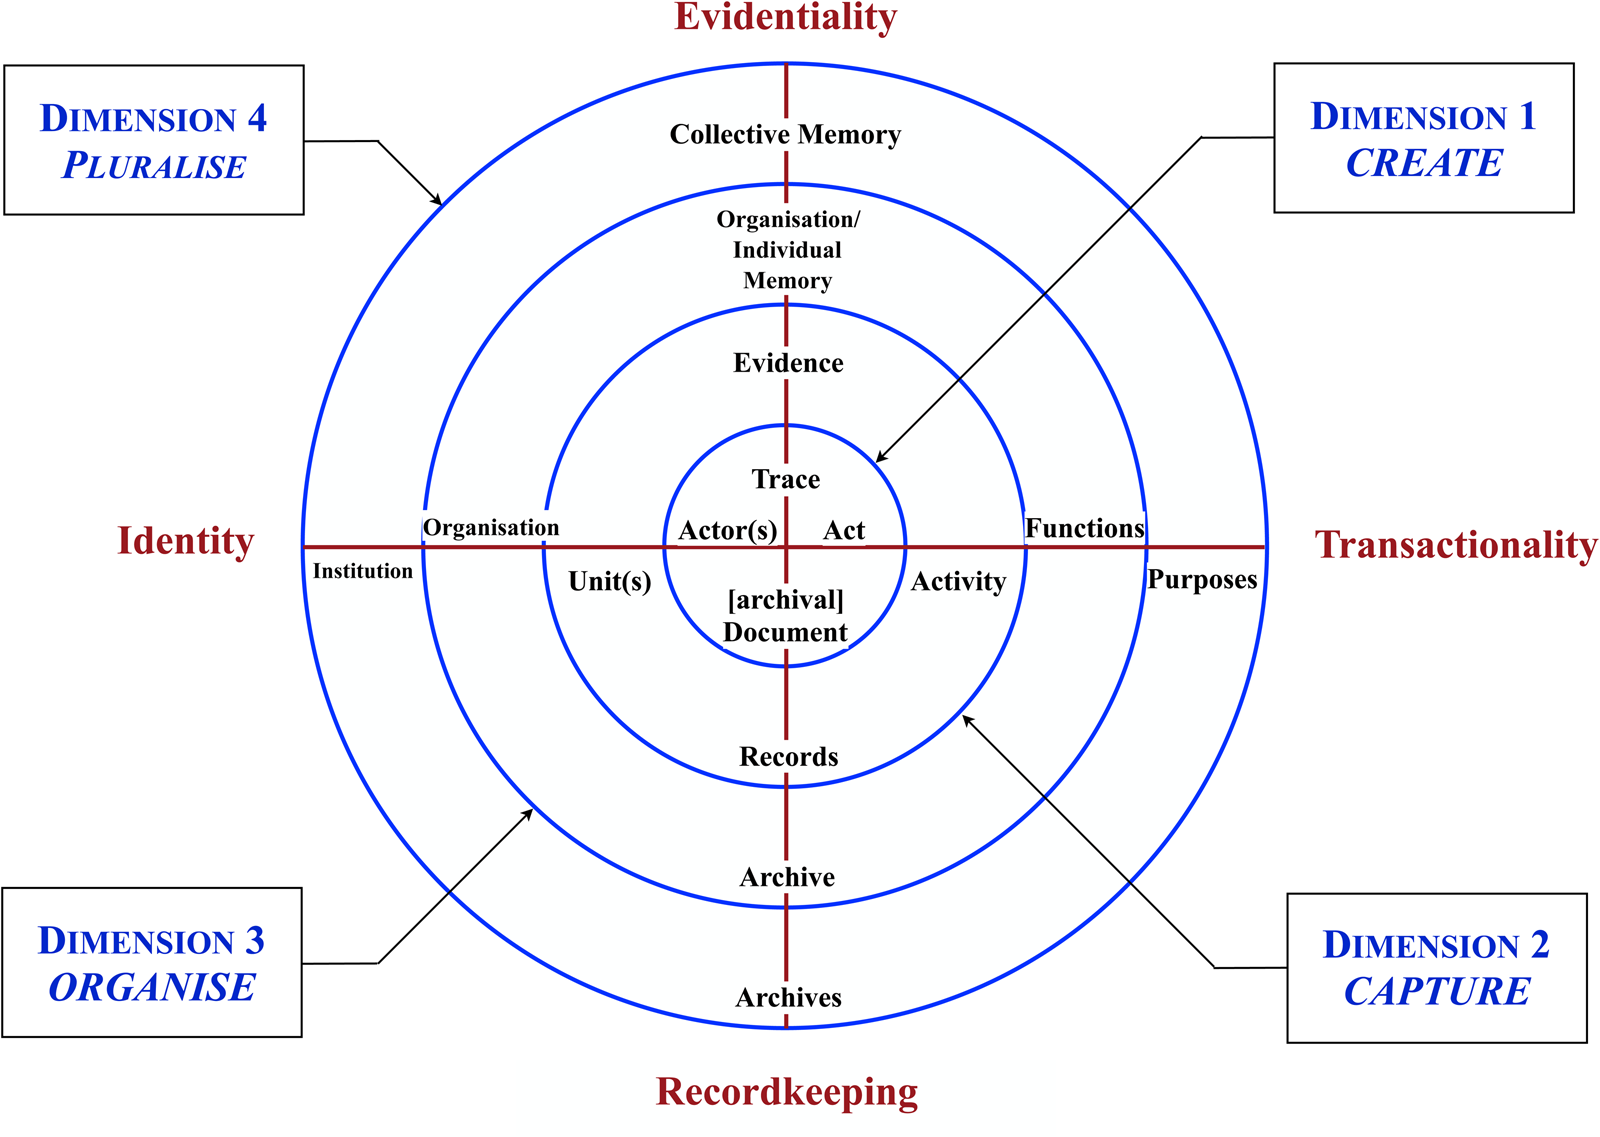
\includegraphics[width=0.95\linewidth, keepaspectratio]{assets/rc3.png}
        \end{tcolorbox}

        \column{0.48\textwidth}
        \begin{premiumbox}[Prinsip Kesatuan]
            \tiny \textbf{Beyond Life Cycle:} Berbeda dengan teori klasik, Continuum Model menegaskan bahwa arsip digital adalah satu kesatuan sejak diciptakan hingga memori korporat.
            \begin{itemize}
                \tiny
                \item \textbf{Create:} Transaksi awal (BAST/SPK).
                \item \textbf{Capture:} Validasi dalam sistem.
                \item \textbf{Organize:} Klasifikasi \& Metadata.
                \item \textbf{Pluralize:} Memori Kolektif \& Audit.
            \end{itemize}
        \end{premiumbox}
        \begin{orangebox}[Strategic Insight]
            \tiny Model ini menjamin bahwa setiap data yang divalidasi di awal (\textit{D-1}) akan tetap sah secara hukum hingga puluhan tahun mendatang (\textit{D-4}).
        \end{orangebox}
    \end{columns}
    \vfill
    \hfill{\fontsize{4}{5}\selectfont\color{gray}Upward, F. (1996). Structuring the Records Continuum. Monash University.}\hspace{1em}
\end{frame}

% SLIDE 11: METODOLOGI (7 DOMAIN)
\begin{frame}{Metodologi: \\ Kerangka Evaluasi 7 Domain Terintegrasi}
    \begin{columns}
        \column{0.5\textwidth}
        \begin{premiumbox}[Standar Global \& Nasional]
            \small
            Kerangka diagnostik yang menggabungkan standar \textbf{ISO, NIST, PARBICA}, serta regulasi nasional (\textbf{PP 71/2019 \& ANRI}).
            \begin{itemize}
                \item Fokus pada Kesiapan (\textit{Readiness}).
                \item Diagnosa 7 Domain Strategis.
            \end{itemize}
        \end{premiumbox}
        
        \column{0.5\textwidth}
        \textbf{7 Domain Evaluasi (Skala 1--5)}
        \vspace{0.2cm}
        \tiny
        \begin{enumerate}
            \item \textbf{Kebijakan:} Dasar hukum di titik transaksi.
            \item \textbf{Tata Kelola:} Otoritas \& RACI Chart.
            \item \textbf{SDM:} Kapasitas \& Budaya kerja.
            \item \textbf{Interoperabilitas:} Komunikasi antar sistem.
            \item \textbf{Proses Bisnis:} Alur tanpa hambatan.
            \item \textbf{Keamanan:} Integritas data.
            \item \textbf{Preservasi:} Kelangsungan jangka panjang.
        \end{enumerate}
    \end{columns}
\end{frame}

% SLIDE 12: POLLING INTERAKTIF (FIX #6: Jeda Interaktif Antar Teori)
\begin{frame}{Refleksi Cepat: Diagnosa Awal Unit Anda}
    \vspace{0.3cm}
    \begin{premiumbox}[Polling Peserta]
        \large
        \centering
        \textit{``Dari 7 domain evaluasi terintegrasi, di domain mana unit kerja Anda merasa \textbf{paling lemah}?''}
    \end{premiumbox}
    \vspace{0.3cm}
    \begin{columns}[T]
        \column{0.48\textwidth}
        \begin{itemize}
            \scriptsize
            \item[$\square$] \textbf{1. Kebijakan} --- Aturan belum sampai ke titik transaksi
            \item[$\square$] \textbf{2. Tata Kelola} --- Tanggung jawab tidak jelas
            \item[$\square$] \textbf{3. SDM} --- Kompetensi digital rendah
            \item[$\square$] \textbf{4. Interoperabilitas} --- Sistem tidak saling bicara
        \end{itemize}
        
        \column{0.48\textwidth}
        \begin{itemize}
            \scriptsize
            \item[$\square$] \textbf{5. Proses Bisnis} --- Masih banyak proses manual
            \item[$\square$] \textbf{6. Keamanan} --- Integritas data belum terjamin
            \item[$\square$] \textbf{7. Preservasi} --- Arsip lama terancam rusak/hilang
        \end{itemize}
    \end{columns}

\end{frame}

% SLIDE 13: THEORY - GOVERNANCE & ISO
\begin{frame}{Landasan Tata Kelola Hukum \& Internasional: ISO 15489}
    \begin{columns}
        \column{0.6\textwidth}
        \begin{premiumbox}[\textit{Information Governance} (Tata Kelola Informasi)]
            \small
            \textit{``Information is a formalized asset that requires executive accountability.''} (ARMA International)
            \vspace{0.2cm}
            \begin{itemize}
                \item Memastikan data tidak hanya sekadar ``Tersimpan'', tapi juga terjamin \textbf{Keabsahan}, \textbf{Perlindungan Hak Akses}, dan \textbf{Nilai Guna Audit}.
            \end{itemize}
        \end{premiumbox}
        \vspace{-0.4cm}
        \begin{greenbox}[ISO 15489-1:2016 --- 4 Karakteristik Arsip Digital]
            \tiny
            \begin{enumerate}
                \item \textbf{Authenticity:} Keaslian pencipta terbukti.
                \item \textbf{Reliability:} Akurat merepresentasikan transaksi.
                \item \textbf{Integrity:} Bebas alterasi (\textit{Hash-lock}).
                \item \textbf{Usability:} Terstruktur \& mudah ditemukan.
            \end{enumerate}
        \end{greenbox}
        
        \column{0.4\textwidth}
        \centering
        \begin{tikzpicture}[scale=0.95]
            % Soft triangle background
            \fill[plnblue!5] (0,2.2) -- (-2,-0.9) -- (2,-0.9) -- cycle;
            \draw[plnblue!20, thick, dashed] (0,2.2) -- (-2,-0.9) -- (2,-0.9) -- cycle;
            
            % Thick colored edges
            \draw[plnblue, line width=2pt] (0, 1.7) -- (-1.5, -0.4);
            \draw[plnorange, line width=2pt] (-1.5, -0.4) -- (1.5, -0.4);
            \draw[plngreen, line width=2pt] (1.5, -0.4) -- (0, 1.7);
            
            % Corner nodes
            \node[circle, fill=plnblue!15, draw=plnblue, line width=1.2pt, minimum size=1.6cm, align=center, font=\scriptsize\bfseries, text=plnblue!80!black] at (0, 1.7) {Accountability};
            \node[circle, fill=plnorange!15, draw=plnorange, line width=1.2pt, minimum size=1.6cm, align=center, font=\scriptsize\bfseries, text=plnorange!80!black] at (-1.5, -0.4) {Integrity};
            \node[circle, fill=plngreen!15, draw=plngreen, line width=1.2pt, minimum size=1.6cm, align=center, font=\scriptsize\bfseries, text=plngreen!80!black] at (1.5, -0.4) {Compliance};
            
            % Prominent TRUST badge in center
            \node[circle, fill=white, draw=plnblue, line width=2pt, inner sep=5pt, font=\bfseries\small, text=plnblue] at (0, 0.5) {TRUST};
        \end{tikzpicture}
    \end{columns}
\end{frame}

% SLIDE 14: STRATEGIC PILLARS
\begin{frame}{3 Pilar Strategis Optimalisasi Prosedur}
    \vspace{0.2cm}
    \begin{columns}[T]
        \column{0.31\textwidth}
        \centering
        \stepicon{plnblue}{1} \\ \textbf{Value-Added Focus} \\
        \vspace{0.1cm}
        \scriptsize Mengeliminasi aktivitas non-produktif.
        
        \column{0.31\textwidth}
        \centering
        \stepicon{plncyan}{2} \\ \textbf{Single Source of Truth} \\
        \vspace{0.1cm}
        \scriptsize Satu input, mengalir otomatis ke seluruh sistem.
        
        \column{0.31\textwidth}
        \centering
        \stepicon{plnorange}{3} \\ \textbf{Rule-Based Routing} \\
        \vspace{0.1cm}
        \scriptsize Persetujuan otomatis berdasarkan kategori risiko.
    \end{columns}
    
    \vspace{0.3cm}
    \centering
    \begin{tikzpicture}[scale=1.0]
        % === Stage 1: Value-Added Focus ===
        \node[rectangle, rounded corners=4pt, draw=plnblue, fill=plnblue!8, minimum width=3cm, minimum height=1.6cm, align=center] (b1) at (0,0) {};
        \node[font=\scriptsize\bfseries, text=plnblue] at (0,0.5) {Value-Added Focus};
        \node[font=\tiny, text=darkgrey] at (0,0.2) {Hapus yang tidak perlu};
        % Mini icon: crossed = waste, plain = value
        \node[fill=red!25, draw=red, minimum size=0.25cm, inner sep=0pt] at (-0.6,-0.2) {};
        \draw[red, very thin] (-0.7,-0.1) -- (-0.5,-0.3);
        \draw[red, very thin] (-0.7,-0.3) -- (-0.5,-0.1);
        \node[fill=plngreen!25, draw=plngreen, minimum size=0.25cm, inner sep=0pt] at (0,-0.2) {};
        \node[fill=red!25, draw=red, minimum size=0.25cm, inner sep=0pt] at (0.6,-0.2) {};
        \draw[red, very thin] (0.5,-0.1) -- (0.7,-0.3);
        \draw[red, very thin] (0.5,-0.3) -- (0.7,-0.1);
        
        \draw[-{Stealth[length=5pt]}, thick, gray!50] (1.6,0) -- (2.2,0);
        
        % === Stage 2: Single Source of Truth ===
        \node[rectangle, rounded corners=4pt, draw=plncyan, fill=plncyan!8, minimum width=3cm, minimum height=1.6cm, align=center] (b2) at (4,0) {};
        \node[font=\scriptsize\bfseries, text=plncyan] at (4,0.5) {Single Source of Truth};
        \node[font=\tiny, text=darkgrey] at (4,0.2) {Input 1×, pakai banyak};
        % Mini icon: hub
        \fill[plncyan!50] (4,-0.15) circle (0.1cm);
        \draw[plncyan, thin] (4,-0.15) -- (3.65,-0.35);
        \draw[plncyan, thin] (4,-0.15) -- (4,-0.4);
        \draw[plncyan, thin] (4,-0.15) -- (4.35,-0.35);
        \fill[plncyan!30] (3.65,-0.35) circle (0.05cm);
        \fill[plncyan!30] (4,-0.4) circle (0.05cm);
        \fill[plncyan!30] (4.35,-0.35) circle (0.05cm);
        
        \draw[-{Stealth[length=5pt]}, thick, gray!50] (5.6,0) -- (6.2,0);
        
        % === Stage 3: Rule-Based Routing ===
        \node[rectangle, rounded corners=4pt, draw=plnorange, fill=plnorange!8, minimum width=3cm, minimum height=1.6cm, align=center] (b3) at (8,0) {};
        \node[font=\scriptsize\bfseries, text=plnorange] at (8,0.5) {Rule-Based Routing};
        \node[font=\tiny, text=darkgrey] at (8,0.2) {Otomatis berdasarkan aturan};
        % Mini icon: decision diamond
        \node[diamond, fill=plnorange!25, draw=plnorange, aspect=1, minimum size=0.35cm, inner sep=0pt] at (8,-0.15) {};
        \draw[-{Stealth[length=4pt]}, plngreen, thin] (8.2,-0.1) -- ++(0.25,0.12);
        \draw[-{Stealth[length=4pt]}, red, thin] (8.2,-0.2) -- ++(0.25,-0.12);
    \end{tikzpicture}
\end{frame}

% SLIDE 15: INVESTIGATIVE PHASE
\begin{frame}{Proses Diagnosa: Mencari Fakta Lapangan}
    \vspace{-0.2cm}
    \begin{premiumbox}[Metode Observasi Lapangan]
        \fontsize{5.5}{6.5}\selectfont
        \begin{tabularx}{\textwidth}{@{} X X X @{}}
            \centering \stepicon{darkgrey}{A}\\ \textbf{Document Shadowing}\\ Melacak pergerakan satu dokumen fisik dari hulu ke hilir untuk melihat hambatan nyata dalam alur distribusi. & 
            \centering \stepicon{darkgrey}{B}\\ \textbf{Log Analysis}\\ Menganalisis jejak digital sistem untuk membandingkan durasi SLA vs fakta riil waktu penyelesaian. & 
            \centering \stepicon{darkgrey}{C}\\ \textbf{Gemba Walk}\\ Observasi langsung di lokasi kerja dan diskusi mendalam mengenai kendala operasional dengan personel terkait.
        \end{tabularx}
    \end{premiumbox}
    
    \begin{columns}[T]
        \column{0.43\textwidth}
        \begin{orangebox}[Pertanyaan Diagnostik Kunci]
            \tiny
            \begin{itemize}
                \item Apakah ada pengetikan ulang data di aplikasi berbeda?
                \item Berapa lama dokumen ``menunggu'' untuk divalidasi?
                \item Apakah setiap modifikasi arsip terekam dalam \textit{Audit Trail}?
            \end{itemize}
        \end{orangebox}

        \column{0.55\textwidth}
        \centering
        \begin{tikzpicture}[scale=0.55, every node/.style={transform shape}]
            % Steps as Boxes
            % Shadowing
            \node[rectangle, rounded corners=6pt, draw=plnblue, fill=plnblue!5, minimum width=3.5cm, minimum height=2.2cm, align=center] (a) at (0,0) {};
            \node[font=\scriptsize\bfseries, text=plnblue] at (0,0.7) {Shadowing};
            \begin{scope}[shift={(0,-0.2)}]
                \draw[thick, plnblue] (-0.3,0) rectangle (0.3,0.5);
                \draw[plnblue] (-0.2,0.4) -- (0.2,0.4); \draw[plnblue] (-0.2,0.3) -- (0.2,0.3);
                \draw[plnorange, very thick] (0.3,0) circle (0.25cm);
                \draw[plnorange, very thick] (0.45,-0.15) -- (0.6,-0.3);
            \end{scope}

            % Log Analysis
            \node[rectangle, rounded corners=6pt, draw=plncyan, fill=plncyan!5, minimum width=3.5cm, minimum height=2.2cm, align=center] (b) at (4.5,2.5) {};
            \node[font=\scriptsize\bfseries, text=plncyan] at (4.5,3.2) {Log Analysis};
            \begin{scope}[shift={(4.5,2.3)}]
                \draw[->, gray] (-0.5,0) -- (0.5,0); \draw[->, gray] (-0.5,0) -- (-0.5,0.7);
                \draw[thick, plncyan] (-0.5,0.1) -- (-0.2,0.5) -- (0.1,0.3) -- (0.4,0.6);
            \end{scope}

            % Gemba Walk
            \node[rectangle, rounded corners=6pt, draw=plnorange, fill=plnorange!5, minimum width=3.5cm, minimum height=2.2cm, align=center] (c) at (9,0) {};
            \node[font=\scriptsize\bfseries, text=plnorange] at (9,0.7) {Gemba Walk};
            \begin{scope}[shift={(9,-0.2)}]
                \draw[thick, plnorange] (0,0.4) circle (0.15cm);
                \draw[thick, plnorange] (0,0.25) -- (0,-0.1);
                \draw[thick, plnorange] (-0.2,0.1) -- (0.2,0.1);
                \draw[plngreen, very thick] (0.4,0) -- (0.5,-0.1) -- (0.7,0.2);
            \end{scope}

            % Arrows
            \draw[-{Stealth[length=8pt]}, line width=1.5pt, gray!30] (1.8,0.5) .. controls (2.5,1.5) .. (3.2,2.0);
            \draw[-{Stealth[length=8pt]}, line width=1.5pt, gray!30] (5.8,2.0) .. controls (6.5,1.5) .. (7.2,0.5);
        \end{tikzpicture}
    \end{columns}
\end{frame}

% SLIDE 16: AS-IS BPMN (FIX #8: Justifikasi BPMN untuk MA)
\begin{frame}{Model BPMN Kondisi Saat Ini (As-Is)}
    \begin{orangebox}[Mengapa MA Perlu Membaca Diagram Ini?]
        \scriptsize MA tidak perlu menggambar diagram dari nol. Namun MA \textbf{wajib mampu membaca dan mengesahkannya} --- BPMN adalah ``Cetak Biru Hukum'' yang menentukan siapa bertanggung jawab apa di setiap titik proses.
    \end{orangebox}
    \vspace{0.1cm}
    \centering
    \resizebox{0.85\textwidth}{!}{%
    \begin{tikzpicture}[node distance=1.2cm and 0.8cm]
    \fill[gray!5] (0.2, 2.5) rectangle (18, 0.6);
    \fill[yellow!4] (0.2, 0.4) rectangle (18, -2.3);
    \fill[gray!5] (0.2, -2.5) rectangle (18, -5.4);
    \draw[gray!30, thick] (0.2, 0.5) -- (18, 0.5);
    \draw[gray!30, thick] (0.2, -2.4) -- (18, -2.4);
    \node[lanelab] at (0.4, 1.6) {Staf Cabang};
    \node[lanelab] at (0.4, -1.0) {Manajer UPT};
    \node[lanelab] at (0.4, -4.0) {Kearsipan};
    \node[startstyle] at (1.5, 1.6) (s1) {Start};
    \node[manual, right=of s1] (m1) {Cetak\\Kontrak\\Rangkap 3};
    \node[manual, right=of m1] (m2) {Isi Form\\Pengantar};
    \node[manual, right=of m2] (m3) {Kirim Kurir\\Internal};
    \node[waiting] at (8.5, -1.0) (w1) {Antrian\\Meja};
    \node[manual, right=of w1] (m4) {Review\\\& TTD\\Basah};
    \node[gateway, right=of m4] (g1) {$\times$};
    \node[manual, right=of g1] (m5) {Stempel\\Basah};
    \node[manual] at (12.5, -4.0) (m6) {Terima\\Fisik};
    \node[manual, right=of m6] (m7) {Catat Buku\\Induk};
    \node[endstyle, right=of m7] (e1) {End};
    \draw[arr] (s1) -- (m1); \draw[arr] (m1) -- (m2); \draw[arr] (m2) -- (m3);
    \draw[arr] (m3.south) -- ++(0,-0.4) -| (w1.north);
    \draw[arr] (w1) -- (m4); \draw[arr] (m4) -- (g1);
    \draw[arrno] (g1.north) -- ++(0,0.8) -| node[above, font=\tiny\itshape, text=red] {Revisi} (m2.south);
    \draw[arr] (g1) -- node[above, font=\tiny\itshape] {OK} (m5);
    \draw[arr] (m5.south) -- ++(0,-0.4) -| (m6.north);
    \draw[arr] (m6) -- (m7); \draw[arr] (m7) -- (e1);
    \node[timelbl, below=0.15cm of w1] {1--3 hari!};
    \node[font=\small\bfseries, text=red!70!black] at (9, -6.5) {SIKLUS MANUAL: 3--5 HARI KERJA};
    \end{tikzpicture}
    }
\end{frame}

% ================================================================
%  TRANSISI: OUTPUT WAJIB BAB 2 (Jembatan Diagnosa -> Desain)
% ================================================================

% SLIDE 17: MATRIKS IDENTIFIKASI AREA OPTIMASI (Output Wajib Bab 2)
\begin{frame}{Output Wajib: Matriks Identifikasi Area Optimasi}
    \vspace{0.1cm}
    \begin{premiumbox}[Jembatan Diagnosa $\rightarrow$ Desain (Kriteria 4.3.1)]
        \scriptsize Hasil diagnosa dari teknik \textit{Fact-Finding} harus dipetakan ke dalam matriks berikut \textbf{sebelum} merancang alur To-Be. Ini adalah input wajib untuk Workshop 1.
    \end{premiumbox}
    \vspace{0.1cm}
    \begin{table}
        \centering
        \tiny
        \begin{tabularx}{\textwidth}{@{} c X X X c @{}}
            \toprule
            \textbf{No} & \textbf{Tahapan Proses} & \textbf{Jenis Hambatan} & \textbf{Potensi Integrasi} & \textbf{Prioritas} \\
            \midrule
            1 & Input data arsip SPK & Duplikasi input dari 2 sistem & Tarik data otomatis dari ERP & \textcolor{red}{\textbf{Tinggi}} \\
            2 & Approval verifikasi & Routing email tanpa SLA & Digital routing + notifikasi & \textcolor{plnorange}{\textbf{Sedang}} \\
            3 & Klasifikasi \& Metadata & Tidak konsisten antar unit & Template metadata + auto-populate & \textcolor{red}{\textbf{Tinggi}} \\
            4 & Penyimpanan arsip & Cetak $\rightarrow$ scan $\rightarrow$ upload & Direct capture dari sistem sumber & \textcolor{plngreen}{\textbf{Rendah}} \\
            \bottomrule
        \end{tabularx}
    \end{table}
    \vspace{0.1cm}
    \begin{orangebox}[Petunjuk Pengisian]
        \scriptsize \textbf{Prioritas} dinilai berdasarkan Tingkat Urgensi vs Effort Implementasi. Fokus pada area \textbf{Tinggi} untuk desain alur kerja di sesi berikutnya. Isi minimal \textbf{4 baris} dari proses riil unit kerja Anda.
    \end{orangebox}
\end{frame}

% ================================================================
%  BAGIAN II: DESAIN \& IMPLEMENTASI (BAB 3--4) --- 20 Menit
% ================================================================

\section{Bagian II:\\Desain \& Implementasi}

% SLIDE 18: DESIGN PRINCIPLES
\begin{frame}{Prinsip Desain Workflow Terintegrasi}
    \vspace{0.2cm}
    \begin{columns}[T]
        \column{0.48\textwidth}
        \begin{premiumbox}[Perspektif Manajerial]
            \scriptsize
            \textbf{Mengapa MA perlu mengawal desain ini?}\\[0.1cm]
            Otomasi adalah \textbf{instrumen pengamanan aset} dan mitigasi risiko hukum. MA yang mengamanatkan desain otomasi secara riil memusnahkan celah intervensi (\textit{tampering/fraud}) data dan mengunci kepatuhan GCG secara \textit{real-time}.
        \end{premiumbox}
        
        \column{0.48\textwidth}
        \begin{orangebox}[3 Prinsip Kunci]
            \scriptsize
            \begin{enumerate}
                \item \textbf{Single Entry, Multiple Use:}\\Eliminasi input ulang $\rightarrow$ nol \textit{human-error}.
                \item \textbf{Rule-Based Routing:}\\Rute validasi dieksekusi terprogram oleh sistem, tanpa intervensi informal.
                \item \textbf{Explicit Exception Handling:}\\Prosedur cadangan (\textit{fallback}) saat jaringan terputus.
            \end{enumerate}
        \end{orangebox}
    \end{columns}
\end{frame}

% SLIDE 18: TO-BE BPMN (FULL)
\begin{frame}{Model BPMN Kondisi Target (To-Be)}
    \centering
    \resizebox{0.95\textwidth}{!}{%
    \begin{tikzpicture}[node distance=1.2cm and 0.8cm]
    \fill[plnblue!4] (0.2, 2.5) rectangle (18, 0.6);
    \fill[plnorange!4] (0.2, 0.4) rectangle (18, -2.3);
    \fill[plnblue!4] (0.2, -2.5) rectangle (18, -5.4);
    \draw[plnblue!20, thick] (0.2, 0.5) -- (18, 0.5);
    \draw[plnblue!20, thick] (0.2, -2.4) -- (18, -2.4);
    \node[lanelab, text=plnblue!80!black] at (0.4, 1.6) {ERP / SAP};
    \node[lanelab, text=plnblue!80!black] at (0.4, -1.0) {Pimpinan};
    \node[lanelab, text=plnblue!80!black] at (0.4, -4.0) {Repositori};
    \node[startstyle_tobe] at (1.5, 1.6) (s2) {Event};
    \node[autostep, right=of s2] (a1) {Auto-Capture\\Metadata\\ERP};
    \node[autostep, right=of a1] (a2) {Generate\\Draft Digital\\(PDF/A)};
    \node[humanstep] at (7.5, -1.0) (h1) {Digital Review\\via E-Office};
    \node[gateway_tobe, right=of h1] (g2) {$\times$};
    \node[humanstep, right=of g2] (h2) {Otorisasi\\TTE};
    \node[autostep] at (12.5, -4.0) (a3) {Hash-Lock\\Immutable};
    \node[autostep, right=of a3] (a4) {Log Audit\\Trail};
    \node[endstyle_tobe, right=of a4] (e2) {Arsip};
    \draw[arr_tobe] (s2) -- (a1); \draw[arr_tobe] (a1) -- (a2);
    \draw[arr_tobe] (a2.south) -- ++(0,-0.4) -| (h1.north);
    \draw[arr_tobe] (h1) -- (g2);
    \draw[arrno] (g2.north) -- ++(0,0.8) -| node[above, font=\tiny\itshape, text=red] {Batal} (a2.south);
    \draw[arrok] (g2) -- node[above, font=\tiny\itshape] {Setuju} (h2);
    \draw[arr_tobe] (h2.south) -- ++(0,-0.4) -| (a3.north);
    \draw[arr_tobe] (a3) -- (a4); \draw[arr_tobe] (a4) -- (e2);
    \node[timelbl_tobe, below=0.15cm of h1] {SLA: 16 Jam};
    \node[font=\small\bfseries, text=green!50!black] at (9, -6.5) {SIKLUS DIGITAL: < 24 JAM};
    \end{tikzpicture}
    }
\end{frame}

% SLIDE 19: PATTERNS OF INTEGRATION
\begin{frame}{3 Pola Integrasi: Elemen Kunci Otomasi}
    \vspace{0.4cm}
    \begin{columns}[T]
        \column{0.31\textwidth}
        \centering
        \stepicon{plnblue}{1} \\ \textbf{\footnotesize Trigger-Based\\Auto-Capture} \\
        \vspace{0.2cm}
        \tiny Begitu status di ERP menjadi \texttt{TECO}, arsip langsung tercipta otomatis tanpa intervensi manual.
        
        \column{0.31\textwidth}
        \centering
        \stepicon{plncyan}{2} \\ \textbf{\footnotesize Parallel Digital\\Routing} \\
        \vspace{0.2cm}
        \tiny Persetujuan dikirim serentak secara paralel. Tidak menunggu distribusi dokumen berantai secara fisik.
        
        \column{0.31\textwidth}
        \centering
        \stepicon{plnorange}{3} \\ \textbf{\footnotesize SLA-Driven\\Escalation} \\
        \vspace{0.2cm}
        \tiny Jika manajer abai $>16$ jam, sistem otomatis mengeskalasi ke atasan langsung sesuai aturan SLA.
    \end{columns}
    
    \vspace{0.3cm}
    \begin{greenbox}[Catatan Arsiparis: \textit{Immutability Lock}]
        \scriptsize Pada \textit{Parallel Routing}, dokumen harus dikunci \textit{read-only}. Revisi diajukan dalam bentuk metadata komentar yang dilacak secara terpusat, bukan mengubah konten dokumen asli.
    \end{greenbox}
\end{frame}

% SLIDE 20: STUDI KASUS ALTERNATIF (FIX #4: BAST Pengadaan)
\begin{frame}{Studi Kasus Alternatif: Arsip BAST E-Procurement}
    \vspace{0.1cm}
    \begin{premiumbox}[Alur Otomasi BAST Pengadaan (7 Langkah)]
        \scriptsize
        \begin{columns}[T]
            \column{0.48\textwidth}
            \begin{enumerate}
                \item \textbf{Pemicu:} Vendor menekan ``Submit Pekerjaan'' di portal E-Procurement.
                \item \textbf{Auto-Generate:} Sistem menyusun draf BAST tanpa diketik manusia.
                \item \textbf{API Transfer:} Draf dikirim ke Sistem E-Office (Tata Persuratan).
                \item \textbf{Review:} Manajer Logistik membuka E-Office, memeriksa substansi draf.
            \end{enumerate}
            
            \column{0.48\textwidth}
            \begin{enumerate}\setcounter{enumi}{4}
                \item \textbf{Gateway:} Ditolak $\rightarrow$ kembali ke vendor. Disetujui $\rightarrow$ TTE.
                \item \textbf{Hash-Lock:} Sistem mengunci arsip BAST permanen (\textit{immutable}).
                \item \textbf{End:} Transaksi BAST tervalidasi digital tanpa satu pun kertas dicetak.
            \end{enumerate}
        \end{columns}
    \end{premiumbox}
    \vspace{0.1cm}
    \begin{orangebox}[Relevansi untuk Peserta dari Unit Pengadaan]
        \scriptsize Integrasi antara E-Procurement dan E-Office mengeliminasi kebutuhan staf mengetik ulang data vendor ke form BAST manual. Seluruh metadata kontrak tertarik otomatis dari portal pengadaan.
    \end{orangebox}
\end{frame}

% SLIDE 21: EXECUTIVE TOLLGATE
\begin{frame}{Validasi Alur: \textit{Executive Tollgate}}
    \vspace{0.2cm}
    \begin{premiumbox}[Daftar Periksa Manajemen Sebelum Implementasi]
        \small
        Sebelum rancangan BPMN disahkan, Manajemen Atas \textbf{wajib} memvalidasi rancangan dengan 4 parameter kritis:
    \end{premiumbox}
    \vspace{0.2cm}
    \begin{table}
        \centering
        \scriptsize
        \begin{tabularx}{\textwidth}{@{} >{\raggedright\arraybackslash}X >{\raggedright\arraybackslash}X c @{}}
            \toprule
            \textbf{Aspek Validasi} & \textbf{Pertanyaan Pemeriksaan} & \textbf{Status} \\
            \midrule
            \textbf{Kelengkapan} & Apakah setiap pemicu memiliki task \& end event yang jelas? & $\square$ \\
            \textbf{Konsistensi} & Apakah semua gateway memiliki jalur \textit{approved} dan \textit{rejected}? & $\square$ \\
            \textbf{Kepatuhan} & Apakah alur memastikan penciptaan arsip sesuai PP 71/2019? & $\square$ \\
            \textbf{Fallback} & Apakah ada prosedur manual digital untuk kondisi sistem \textit{down}? & $\square$ \\
            \bottomrule
        \end{tabularx}
    \end{table}
\end{frame}

% SLIDE 22: WORKSHOP 1 (FIX #3: Aktivitas Workshop)
\begin{frame}{Workshop 1:\\Perancangan Alur Kerja Terintegrasi (20 Menit)}
    \vspace{0.1cm}
    \begin{premiumbox}[Instruksi Aktivitas Kelompok]
        \small
        \begin{enumerate}
            \item Gunakan Matriks Identifikasi Bab 2 sebagai \textit{input}.
            \item Pilih \textbf{1 proses prioritas tinggi} untuk dirancang ulang.
            \item Gambar diagram \textbf{BPMN To-Be} pada lembar kerja yang disediakan.
            \item Lakukan \textbf{validasi silang} dengan kelompok lain menggunakan \textit{Executive Tollgate} (4 parameter).
        \end{enumerate}
    \end{premiumbox}
    \vspace{-0.2cm}
    \begin{columns}[T]
        \column{0.35\textwidth}
        \begin{greenbox}[Alat Bantu Rekomendasi]
            \tiny
            \textbf{Desktop:}\\ Visio, Bizagi Modeler\\
            \textbf{Web:}\\ Draw.io, Lucidchart, Miro
        \end{greenbox}

        \column{0.61\textwidth}
        \begin{orangebox}[Output Wajib]
            \scriptsize
            \begin{tabular}{@{}c l@{}}
                \stepicon{plnorange}{\checkmark} & \textbf{Diagram BPMN 2.0 (To-Be)}\\
                \stepicon{plnorange}{\checkmark} & \textbf{Peta Pemicu Integrasi}\\
            \end{tabular}
            \vspace{0.1cm}
            \centering \tiny \textit{Kriteria Penilaian: 4.3.2}
        \end{orangebox}
    \end{columns}
\end{frame}

% SLIDE 23: SOP EVOLUTION
\begin{frame}{Evolusi Paradigma SOP}
    \centering
    \begin{tikzpicture}[
        scale=0.58, every node/.style={transform shape},
        dimnode/.style={rounded rectangle, fill=DimCenter, text=white, font=\bfseries, align=center, minimum width=4.5cm, minimum height=0.9cm, drop shadow={opacity=0.2, shadow xshift=0pt, shadow yshift=-2pt}},
        leftnode/.style={rectangle, draw=NodeLeftBorder, thick, dashed, rounded corners, fill=NodeLeftBg, align=center, minimum width=6cm, minimum height=1cm, text=TitleDark},
        rightnode/.style={rectangle, fill=NodeRightBg, align=center, font=\bfseries\color{PilarRight}, rounded corners, minimum width=6cm, minimum height=1cm, drop shadow={opacity=0.2, shadow xshift=0pt, shadow yshift=-2pt}},
        arrow/.style={-{Stealth[scale=1.2]}, thick, draw=PilarRight},
        dashline/.style={dashed, thick, draw=NodeLeftBorder}
    ]

    % --- PHASE HEADERS ---
    \node[align=center] (headleft) at (-6, 0.5) {\Large\bfseries\color{PilarLeft} SOP KONVENSIONAL \\ \large\color{TitleSub} (Fragmentasi \& Manual)};
    \node[align=center] (headright) at (6, 0.5) {\Large\bfseries\color{PilarRight} SOP DIGITAL TERINTEGRASI \\ \large\color{CircuitColor} (Orkestrasi \& Otonom)};

    % --- RIGHT PILLAR BACKGROUND ---
    \fill[NodeRightBg!40!white, rounded corners=15pt, draw=CircuitColor!50, dashed, thick] (2.5, -0.5) rectangle (10.5, -8.2);

    % --- DIMENSION 1 ---
    \node[dimnode] (dim1) at (0, -1.5) {FOKUS EKOSISTEM};
    \node[leftnode] (L1) at (-6, -1.5) {Interaksi fisik antar-manusia};
    \node[rightnode] (R1) at (6, -1.5) {Orkestrasi sistem \& manusia};
    \draw[dashline] (L1) -- (dim1); \draw[arrow] (dim1) -- (R1);

    % --- DIMENSION 2 ---
    \node[dimnode] (dim2) at (0, -3.0) {INISIATOR PROSES};
    \node[leftnode] (L2) at (-6, -3.0) {Inisiatif manual oleh staf};
    \node[rightnode] (R2) at (6, -3.0) {System-Event Trigger otomatis};
    \draw[dashline] (L2) -- (dim2); \draw[arrow] (dim2) -- (R2);

    % --- DIMENSION 3 ---
    \node[dimnode] (dim3) at (0, -4.5) {VALIDASI NASKAH};
    \node[leftnode] (L3) at (-6, -4.5) {Tanda tangan basah \& stempel};
    \node[rightnode] (R3) at (6, -4.5) {Audit Trail \& TTE};
    \draw[dashline] (L3) -- (dim3); \draw[arrow] (dim3) -- (R3);

    % --- DIMENSION 4 ---
    \node[dimnode] (dim4) at (0, -6.0) {MANAJEMEN RISIKO};
    \node[leftnode] (L4) at (-6, -6.0) {Reaktif, bergantung daya ingat};
    \node[rightnode] (R4) at (6, -6.0) {Preventif, immutable \& real-time};
    \draw[dashline] (L4) -- (dim4); \draw[arrow] (dim4) -- (R4);

    % --- DIMENSION 5 ---
    \node[dimnode] (dim5) at (0, -7.5) {PENEMPATAN ARSIP};
    \node[leftnode] (L5) at (-6, -7.5) {Menunggu petugas pasca dinas};
    \node[rightnode] (R5) at (6, -7.5) {Preservation by design; otonom};
    \draw[dashline] (L5) -- (dim5); \draw[arrow] (dim5) -- (R5);

    % --- CIRCUIT SPINE ---
    \draw[line width=2pt, CircuitColor] (10, -1) -- (10, -8);
    \foreach \y in {-1.5, -3.0, -4.5, -6.0, -7.5}
        \fill[PilarRight] (10, \y) circle (4pt);

    % --- FOUNDATION (INSIGHT) ---
    \node[rectangle, rounded corners=12pt, fill=FoundBg1, minimum width=21cm, minimum height=3.5cm, drop shadow={opacity=0.3, shadow xshift=0pt, shadow yshift=-4pt}] (found) at (0, -10.5) {};
    \node[align=left, anchor=north west] at ([xshift=1cm, yshift=-0.5cm]found.north west) {
        \Large\bfseries\color{FoundTitle} SOP SEBAGAI PROTOKOL KORPORAT
    };
    \node[align=left, anchor=north west, text=white, text width=19.5cm] at ([xshift=1cm, yshift=-1.3cm]found.north west) {
        \large Bukan lagi sekadar dokumen panduan statis (\textit{\color{gray!50}User Guide}), melainkan arsitektur pengikat yang menjamin \\[0.1cm]
        \large \textbf{\color{FoundHighlight} SLA}, \textbf{\color{FoundHighlight} Orkestrasi Alur Kerja}, dan \textbf{\color{FoundHighlight} Akuntabilitas Keputusan} secara terotomatisasi.
    };

    \end{tikzpicture}
\end{frame}

% SLIDE 24: 8 KOMPONEN WAJIB SOP
\begin{frame}{Struktur SOP Digital Terintegrasi: 8 Komponen Wajib}
    \vspace{0.2cm}
    \begin{columns}[T]
        \column{0.48\textwidth}
        \scriptsize
        \begin{enumerate}
            \item \textbf{Tujuan \& Lingkup Interoperabilitas:}\\Batasan penarikan data antar-sistem.
            \item \textbf{Dasar Hukum:}\\UU ITE, PP 71/2019, Perka ANRI.
            \item \textbf{Definisi Digital:}\\Token, Hash, RBAC, Metadata.
            \item \textbf{Peran + System Custodian:}\\Mengakui \textbf{Sistem} sebagai entitas pengawasan.
        \end{enumerate}
        
        \column{0.48\textwidth}
        \scriptsize
        \begin{enumerate}\setcounter{enumi}{4}
            \item \textbf{Klasifikasi, Retensi \& Akses:}\\Matriks kodifikasi wajib \& RBAC.
            \item \textbf{Alur Kerja + Trigger Points:}\\Desain pemicu sistem \& rute paralel.
            \item \textbf{Exception \& Fallback:}\\Protokol pemulihan saat \textit{downtime}.
            \item \textbf{Lampiran Teknis:}\\Peta database, log audit trail, matriks metadata.
        \end{enumerate}
    \end{columns}
    \vspace{0.2cm}
    \begin{greenbox}[Evolusi, Bukan Revolusi Format]
        \scriptsize Format SOP (Tujuan, Referensi, Definisi, Uraian Langkah) tetap identik dengan pedoman korporat. Yang berubah adalah \textbf{kualitas isi tiap bab}, dari kendali manual ke kendali sistem komputasi terpusat.
    \end{greenbox}
\end{frame}

% SLIDE 25: METADATA EVIDENCE FRAMEWORK
\begin{frame}{14 Field Metadata: Kerangka Bukti Hukum}
    \vspace{0.2cm}
    \begin{columns}
        \column{0.48\textwidth}
        \begin{premiumbox}[Evidence \& Compliance (Otentisitas)]
            \tiny
            \begin{itemize}
                \item \texttt{DOC\_ID}: ID Unik Dokumen.
                \item \texttt{TIMESTAMP}: Waktu mutlak (ISO 8601).
                \item \texttt{HASH}: Segel digital (SHA-256).
                \item \texttt{CREATOR\_ROLE}: Jabatan penandatangan (RBAC).
                \item \texttt{AUDIT\_LOG\_ID}: Jejak riwayat sistem.
                \item \texttt{CLASSIFICATION}: Vital/Internal/Rahasia.
                \item \texttt{RETENTION\_RULE}: Jadwal JRA otomatis.
            \end{itemize}
        \end{premiumbox}
        
        \column{0.48\textwidth}
        \begin{orangebox}[Discovery \& Retrieve (Nilai Guna)]
            \tiny
            \begin{itemize}
                \item \texttt{ASSET\_ID}: Referensi aset (SAP-PM).
                \item \texttt{WO\_REF}: Referensi Work Order.
                \item \texttt{CONTRACT\_REF}: No. Kontrak Korporat.
                \item \texttt{LOCATION}: Kode GIS operasional.
                \item \texttt{CREATOR\_UNIT}: Unit pencipta arsip.
                \item \texttt{CONTENT\_DESC}: Ringkasan isi naskah.\textsuperscript{*}
                \item \texttt{SEARCH\_TAGS}: Kata kunci pencarian.\textsuperscript{*}
            \end{itemize}
            \vspace{0.1cm}
            \textsuperscript{*}\textit{Semi-Mandatory (Enhancement)}
        \end{orangebox}
    \end{columns}
\end{frame}

% SLIDE 26: THE METADATA JOURNEY (Exploded View - FULL 14 FIELDS)
\begin{frame}{The Metadata Journey: Struktur Berlapis Arsip Digital}
    \centering
    \resizebox{0.55\textwidth}{!}{%
    \begin{tikzpicture}
        % Background concentric circles
        \draw[dashed, plnblue!20, fill=plnblue!5] (0,0) circle (3.0cm);
        \draw[dashed, plnorange!20, fill=plnorange!5] (0,0) circle (2.2cm);
        \draw[dashed, plncyan!20, fill=plncyan!5] (0,0) circle (1.4cm);

        % Central Document
        \node[docstyle, minimum height=2.2cm, minimum width=1.6cm] (paper) at (0,0) {};
        \node[font=\bfseries\fontsize{5}{6}\selectfont, color=plnblue] at (0,0.8) {KONTEN};
        \node[font=\fontsize{4}{5}\selectfont, color=darkgrey, text width=1.2cm, align=center] at (0,0) {Isi Dokumen:\\BAST / SPK};
        
        % Layer 1: Evidence (4 nodes) - plncyan
        \node[meta=plncyan] at (45:1.4cm) {HASH\\(SHA-256)};
        \node[meta=plncyan] at (135:1.4cm) {TIME\\STAMP};
        \node[meta=plncyan] at (225:1.4cm) {DOC\\ID};
        \node[meta=plncyan] at (315:1.4cm) {AUDIT\\LOG};
        
        % Layer 2: Context (5 nodes) - plnorange
        \node[meta=plnorange] at (0:2.2cm) {ASSET\\ID};
        \node[meta=plnorange] at (72:2.2cm) {WO\\REF};
        \node[meta=plnorange] at (144:2.2cm) {CONTR\\REF};
        \node[meta=plnorange] at (216:2.2cm) {GIS\\LOC};
        \node[meta=plnorange] at (288:2.2cm) {UNIT\\ID};
        
        % Layer 3: Governance (5 nodes) - plnblue
        \node[meta=plnblue] at (30:3.0cm) {CLASSIFY};
        \node[meta=plnblue] at (102:3.0cm) {RETENTION};
        \node[meta=plnblue] at (174:3.0cm) {USER\\ROLE};
        \node[meta=plnblue] at (246:3.0cm) {DESC};
        \node[meta=plnblue] at (318:3.0cm) {TAGS};

        % Legend
        \node[anchor=west, plncyan!80!black, font=\bfseries\fontsize{5}{6}\selectfont] at (3.8,1.0) {LAYER 1: EVIDENTIAL (4)};
        \node[anchor=west, plnorange!80!black, font=\bfseries\fontsize{5}{6}\selectfont] at (3.8,0.5) {LAYER 2: CONTEXTUAL (5)};
        \node[anchor=west, plnblue!80!black, font=\bfseries\fontsize{5}{6}\selectfont] at (3.8,0.0) {LAYER 3: GOVERNANCE (5)};
        
    \end{tikzpicture}%
    }
    \vspace{-0.1cm}
    \begin{center}
        \begin{minipage}{0.7\textwidth}
            \begin{premiumbox}[Insight Imersif: Total 14 Field Metadata]
                \scriptsize \textbf{Data Is the New Document:}\\ Arsip digital bukan hanya gambar, melainkan paket data 14-field terstruktur yang menjamin keamanan dan keterlacakan aset PLN sepanjang masa.
            \end{premiumbox}
        \end{minipage}
    \end{center}
\end{frame}

% SLIDE 27: LEGAL STANDING
\begin{frame}{Keabsahan Hukum: TTE vs TTD Basah}
    \begin{columns}
        \column{0.6\textwidth}
        \begin{premiumbox}[PP No. 71 Tahun 2019 (Pasal 14--16)]
            \small
            \textbf{TTE Tersertifikasi} memiliki kekuatan hukum yang setara dengan tanda tangan basah secara absolut.
            \begin{itemize}
                \scriptsize
                \item \textbf{Autentisitas:} Terhubung hanya ke pemilik.
                \item \textbf{Integritas:} Setiap perubahan terdeteksi.
                \item \textbf{Nirsangkal:} Tidak bisa disangkal.
            \end{itemize}
        \end{premiumbox}
        \vspace{0.1cm}
        \begin{greenbox}[Implikasi dalam SOP]
            \scriptsize
            \textit{``Setiap persetujuan digital memiliki status final secara hukum. Perubahan status arsip pasca-validasi wajib direkam dalam log yang tidak dapat dihapus (immutable).''}
        \end{greenbox}
        
        \column{0.4\textwidth}
        \centering
        \stepicon{plngreen}{\checkmark} \\[0.2cm]
        \small \textbf{VALID \& SECURE}\\[0.3cm]
        \scriptsize
        Kepatuhan meliputi:\\
        UU ITE\\
        PP 71/2019 (PSTE)\\
        Perka ANRI No. 6/2021
    \end{columns}
\end{frame}

% SLIDE 28: DIGITAL SIGNATURE TRUST-CHAIN
\begin{frame}{Mekanisme Keamanan: Digital Signature Trust-Chain}
    \begin{columns}
        \column{0.55\textwidth}
        \centering
        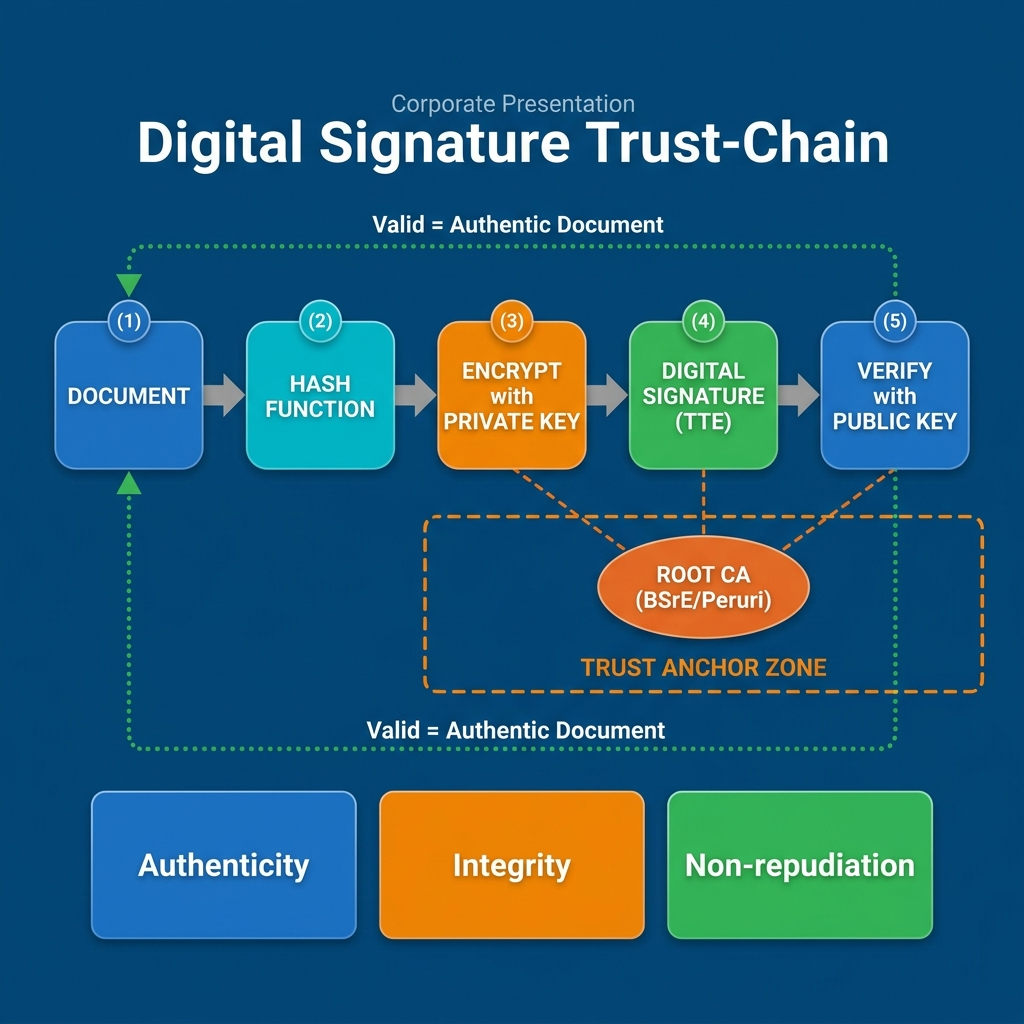
\includegraphics[width=0.85\textwidth,keepaspectratio]{trust_chain.png}

        \column{0.45\textwidth}
        \begin{premiumbox}[Kekuatan Hukum Digital]
            \scriptsize
            Setiap tahap dijamin oleh \textbf{Root CA terakreditasi}:
            \begin{itemize}
                \tiny
                \item \textbf{Authenticity:} Identitas terikat sertifikat unik.
                \item \textbf{Integrity:} Hash menjamin isi tidak berubah.
                \item \textbf{Non-repudiation:} Bukti kriptografis final.
            \end{itemize}
        \end{premiumbox}
        \begin{orangebox}[Strategic Impact]
            \tiny Menghilangkan keraguan legalitas arsip digital dalam proses audit eksternal BPK/BPKP.
        \end{orangebox}
    \end{columns}
    \vfill
    \hfill{\fontsize{4}{5}\selectfont\color{gray}Ref: PP No. 71/2019 tentang PSTE; UU ITE. Adaptasi visual untuk PT PLN (Persero).}\hspace{1em}
\end{frame}
% SLIDE 29: BLOCKCHAIN HASH CHAIN
\begin{frame}{Menjamin Integritas:\\Blockchain Hash Chain \& Immutability}
    \begin{columns}
        \column{0.55\textwidth}
        \centering
        \begin{tcolorbox}[colback=white, colframe=plnblue!15, boxrule=0.5pt, arc=2pt, outer arc=2pt, left=2pt, right=2pt, top=2pt, bottom=2pt, boxsep=0pt, width=0.95\linewidth, drop shadow]
            \centering
            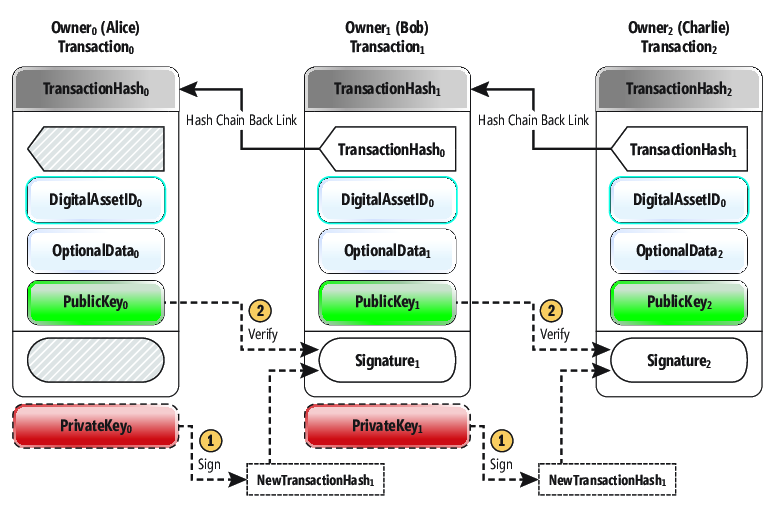
\includegraphics[width=0.9\linewidth,keepaspectratio]{assets/Blockchain_Hash_Chain.png}
        \end{tcolorbox}

        \column{0.45\textwidth}
        \begin{premiumbox}[Mekanisme Immutability]
            \scriptsize
            Bagaimana sistem mengunci keabsahan arsip:
            \begin{itemize}
                \tiny
                \item \textbf{Keterhubungan Kriptografis:} Setiap blok data membawa identitas (*hash*) dari data sebelumnya.
                \item \textbf{Segel Kepercayaan:} Perubahan pada satu byte data akan merusak seluruh rantai validasi.
                \item \textbf{Bukti Manipulasi:} Upaya manipulasi akan terdeteksi seketika oleh sistem audit.
            \end{itemize}
        \end{premiumbox}
        \begin{greenbox}[Kedaulatan Data]
            \tiny Menjamin bahwa arsip yang tercipta hari ini akan tetap memiliki bukti otentisitas yang sama hingga puluhan tahun mendatang.
        \end{greenbox}
    \end{columns}
    \vfill
    \hfill{\fontsize{4}{5}\selectfont\color{gray}Konsep Kriptografi: Rantai Hash untuk Audit Trail yang Tidak Dapat Dimanipulasi. Ref: Nakamoto, S. (2008). Bitcoin: A Peer-to-Peer Electronic Cash System.}\hspace{1em}
\end{frame}


% ================================================================
%  BAGIAN III: ANALISIS ROI \& TINDAK LANJUT (BAB 5--6) --- 10 Menit
% ================================================================

\section{Bagian III:\\ROI \& Tindak Lanjut}

% SLIDE 29: KPI FRAMEWORK
\begin{frame}{Metodologi Pengukuran: \textit{Time-Cost-Risk Saving}}
    \vspace{0.2cm}
    \begin{columns}[T]
        \column{0.53\textwidth}
        \begin{premiumbox}[Kerangka Trifecta]
            \scriptsize
            \begin{itemize}
                \item \textcolor{plnblue}{\textbf{Time Saving:}} Pemangkasan waktu tunggu \& durasi proses.
                \item \textcolor{plnorange}{\textbf{Cost Saving:}} Reduksi pengeluaran riil (cetak, depo arsip).
                \item \textcolor{plngreen}{\textbf{Risk Saving:}} Perlindungan sanksi hukum \& kehilangan data.
            \end{itemize}
        \end{premiumbox}
        
        \column{0.43\textwidth}
        \begin{orangebox}[Formula ROI]
            \tiny
            \textbf{Productivity Gain:}\\
            $\Delta$Waktu $\times$ Volume $\times$ Biaya/Jam\\[0.1cm]
            \textbf{Cost Avoidance:}\\
            Eliminasi cetak ulang, kurir, sewa depo arsip.\\[0.1cm]
            \textbf{Risk Reduction:}\\
            Denda litigasi \& temuan audit (BPK/BPKP).
            \vfill
            \textbf{Time} \& \textbf{Cost} = Efisiensi Hari Ini\\
            \textbf{Risk} = Keamanan Masa Depan
        \end{orangebox}
    \end{columns}
\end{frame}

% SLIDE 29: KPI & DASHBOARD
\begin{frame}{4 Indikator Kinerja Utama (KPI)}
    \vspace{0.3cm}
    \begin{columns}[T]
        \column{0.24\textwidth}
        \centering
        \stepicon{plnblue}{1} \\ \textbf{Waktu Siklus} \\ \tiny (\textit{Cycle Time}) \\[0.1cm]
        \scriptsize Target: $\downarrow$ 40--60\%\\
        (5 hari $\rightarrow$ 1--2 hari)
        
        \column{0.24\textwidth}
        \centering
        \stepicon{plncyan}{2} \\ \textbf{Ketepatan Awal} \\ \tiny (\textit{First-Time Accuracy}) \\[0.1cm]
        \scriptsize Target: $\uparrow$ $\geq$90\%\\
        Lolos validasi tanpa revisi
        
        \column{0.24\textwidth}
        \centering
        \stepicon{plnorange}{3} \\ \textbf{Waktu Temu Kembali} \\ \tiny (\textit{Retrieval Speed}) \\[0.1cm]
        \scriptsize Target: $<$ 30 Detik\\
        (query digital)
        
        \column{0.24\textwidth}
        \centering
        \stepicon{plngreen}{4} \\ \textbf{Kepatuhan Prosedur} \\ \tiny (\textit{Compliance Rate}) \\[0.1cm]
        \scriptsize Target: $\geq$ 95\%\\
        SLA + Retensi + Audit
    \end{columns}
    \vspace{0.1cm}
    \begin{premiumbox}[Kriteria Kepatuhan]
        \tiny
        \begin{itemize}
            \item \textbf{Arsip Digital:} Audit trail, TTE, hash (\textit{immutable}), metadata otomatis.
            \item \textbf{Arsip Hibrida:} Sinkronisasi fisik-digital \& label retensi JRA.
        \end{itemize}
    \end{premiumbox}
\end{frame}

% SLIDE 30: EFFICIENCY HEATMAP (Before vs. After)
\begin{frame}{Efficiency Heatmap: Transformasi Kecepatan Layanan}
    \vspace{0.2cm}
    \begin{premiumbox}[Analisis Waktu Tunggu Proses Bisnis Kearsipan]
        \scriptsize Perbandingan durasi siklus antara metode konvensional (Manual) dengan metode terintegrasi (Digital).
    \end{premiumbox}
    \vspace{0.4cm}
    \centering
    \resizebox{0.9\textwidth}{!}{%
    \begin{tikzpicture}[
        barstyle/.style={rectangle, rounded corners=2pt, minimum height=0.8cm, draw=white, line width=1pt},
        labelstyle/.style={font=\tiny\bfseries, text=white}
    ]
        % Timeline Scale
        \draw[thick, gray!30, -Stealth] (0, 2.5) -- (12, 2.5) node[right, font=\tiny] {Hari Kerja};
        \foreach \x in {0,1,2,3,4,5} \node[font=\tiny, gray] at (\x*2, 2.8) {\x};

        % AS-IS (Manual)
        \node[anchor=west, font=\small\bfseries, color=plnblue] at (-4, 1.2) {MANUAL (As-Is)};
        \node[barstyle, fill=plnblue!40, minimum width=2cm, anchor=west] (b1) at (0, 1.2) {};
        \node[labelstyle] at (b1.center) {Drafting};
        
        \node[barstyle, fill=red!60, minimum width=3cm, anchor=west] (b2) at (2, 1.2) {};
        \node[labelstyle] at (b2.center) {Cetak/Kurir};
        
        \node[barstyle, fill=red!80, minimum width=4cm, anchor=west] (b3) at (5, 1.2) {};
        \node[labelstyle] at (b3.center) {Antrian Persetujuan};
        
        \node[barstyle, fill=plnblue!60, minimum width=1cm, anchor=west] (b4) at (9, 1.2) {};
        \node[labelstyle] at (b4.center) {Scan};
        
        % TO-BE (Digital)
        \node[anchor=west, font=\small\bfseries, color=plngreen] at (-4, -0.5) {DIGITAL (To-Be)};
        \node[barstyle, fill=plngreen!60, minimum width=0.8cm, anchor=west] (t1) at (0, -0.5) {};
        \node[labelstyle] at (t1.center) {Auto};
        
        \node[barstyle, fill=plngreen!80, minimum width=1.5cm, anchor=west] (t2) at (0.8, -0.5) {};
        \node[labelstyle] at (t2.center) {Digital Appr.};
        
        \node[barstyle, fill=plncyan!70, minimum width=1.1cm, anchor=west] (t3) at (2.3, -0.5) {};
        \node[labelstyle] at (t3.center) {Simpan};
        
        % Efficiency Arrow
        \draw[Stealth-Stealth, plnorange, line width=2pt] (10.5, 1.2) -- (10.5, -0.5) node[midway, right, font=\bfseries\small] {Efisiensi $>$ 75\%};
        
        % Legend
        \fill[red!70] (0, -2.2) rectangle (0.3, -2.5); \node[right, font=\tiny] at (0.3, -2.35) {Non-Value Added (Waiting/Manual)};
        \fill[plngreen!70] (5, -2.2) rectangle (5.3, -2.5); \node[right, font=\tiny] at (5.3, -2.35) {Value Added (Automated)};
    \end{tikzpicture}%
    }
\end{frame}


% SLIDE 31: BALANCED SCORECARD (BSC)
\begin{frame}{Kerangka Kerja Strategis: Balanced Scorecard (BSC)}
    \begin{columns}
        \column{0.55\textwidth}
        \centering
        \begin{tcolorbox}[colback=white, colframe=plnblue!15, boxrule=0.5pt, arc=2pt, outer arc=2pt, left=2pt, right=2pt, top=2pt, bottom=2pt, boxsep=0pt, width=0.95\linewidth, drop shadow]
            \centering
            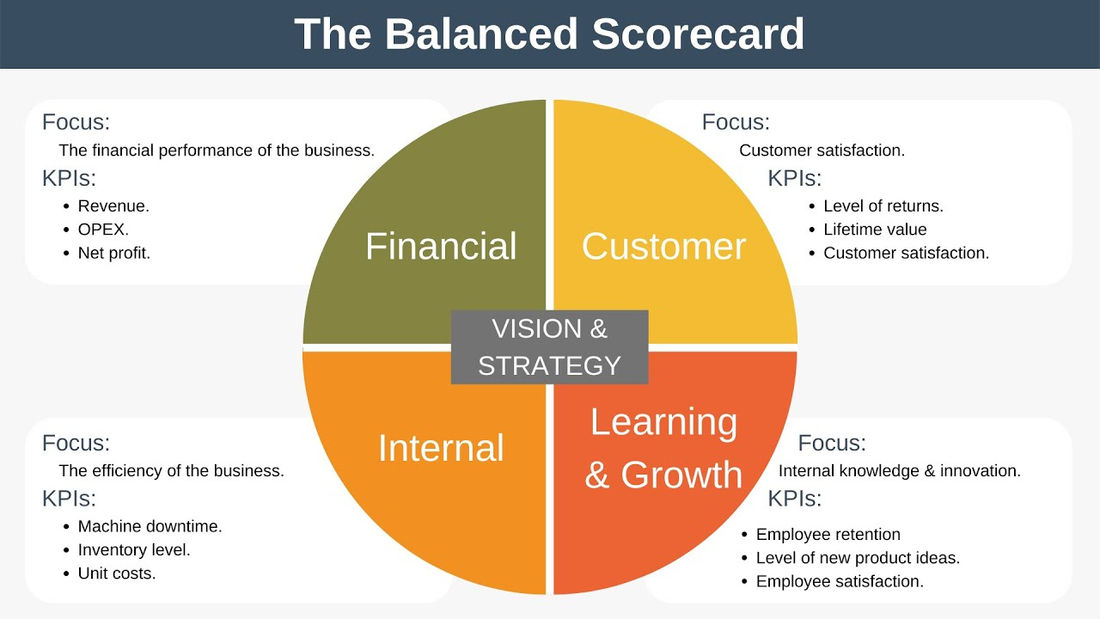
\includegraphics[width=0.9\linewidth,keepaspectratio]{assets/Balanced_Scorecard.png}
        \end{tcolorbox}

        \column{0.45\textwidth}
        \begin{premiumbox}[Penjabaran Metrik Kearsipan]
            \scriptsize
            Penerapan 4 perspektif BSC dalam dashboard:
            \begin{itemize}
                \tiny
                \item \textbf{Financial:} Penghematan biaya ruang \& operasional melalui eliminasi kertas (\textit{Cost Saved}).
                \item \textbf{Customer:} Kecepatan \& ketepatan layanan data bagi unit kerja (\textit{Accuracy Rate}).
                \item \textbf{Internal Process:} Efisiensi siklus hidup dokumen dari penciptaan hingga preservasi (\textit{Cycle Time}).
                \item \textbf{Learning \& Growth:} Kepatuhan standar kearsipan \& indeks literasi digital (\textit{Compliance Status}).
            \end{itemize}
        \end{premiumbox}
        \begin{orangebox}[Strategy-Driven Dashboard]
            \tiny Menjamin bahwa setiap angka yang dipantau oleh eksekutif memiliki korelasi langsung dengan pencapaian visi strategis korporat.
        \end{orangebox}
    \end{columns}
    \vfill
    \hfill{\fontsize{4}{5}\selectfont\color{gray}Ref: Kaplan, R.S. \& Norton, D.P. (2004). Strategy Maps: Converting Intangible Assets into Tangible Outcomes.}\hspace{1em}
\end{frame}

% SLIDE 32: DASHBOARD MOCKUP (Real-Time KPI Tracker)
\begin{frame}{Dashboard Executive: Real-Time KPI Tracker}
    \centering
    \fontsize{5}{6}\selectfont \color{gray} *Seluruh data di bawah ini adalah data simulasi untuk kepentingan diklat
    \vspace{0.1cm}
    \centering
    \resizebox{0.78\textwidth}{!}{%
    \begin{tikzpicture}[
        card/.style={rectangle, rounded corners=3pt, fill=white, draw=gray!20, minimum width=3cm, minimum height=1.6cm, drop shadow={opacity=0.1}},
        title/.style={font=\tiny\bfseries, color=gray},
        value/.style={font=\small\bfseries, color=plnblue}
    ]
        % Dashboard Background
        \fill[gray!5, rounded corners=5pt] (-5.5, -2.6) rectangle (5.5, 2.6);
        \node[font=\tiny\bfseries, color=plnblue] at (-2.8, 2.3) {PLN ARCHIVE PERFORMANCE DASHBOARD};
        
        % Metric Cards (Top Row)
        \node[card] (c1) at (-3.6, 1.2) {};
        \node[title] at (-3.6, 1.7) {AVERAGE CYCLE TIME};
        \node[value] at (-3.6, 1.2) {1.2 Days};
        \node[font=\tiny, color=plngreen] at (-3.6, 0.8) {$\downarrow$ 76\% vs Manual};

        \node[card] (c2) at (0, 1.2) {};
        \node[title] at (0, 1.7) {ACCURACY RATE};
        \node[value] at (0, 1.2) {94.2\%};
        \node[font=\tiny, color=plngreen] at (0, 0.8) {$\uparrow$ 12\% Goal};

        \node[card] (c3) at (3.6, 1.2) {};
        \node[title] at (3.6, 1.7) {COST SAVED (YTD)};
        \node[value] at (3.6, 1.2) {Rp 1.4B};
        \node[font=\tiny, color=plnorange] at (3.6, 0.8) {Target: Rp 2B};

        % Charts (Middle/Bottom)
        \fill[white, rounded corners=3pt, draw=gray!10] (-5.2, -2.2) rectangle (1.5, 0.0);
        \node[title, anchor=west] at (-5, -0.3) {Document Volume by Unit};
        % Mini Bar Chart
        \foreach \h/\x/\u in {1.0/-4.5/Dist, 0.7/-3.5/Trans, 1.4/-2.5/Gen, 0.5/-1.5/Corp} {
            \fill[plnblue!70] (\x, -1.9) rectangle (\x+0.5, -1.9+\h);
            \node[rotate=45, font=\fontsize{3}{4}\selectfont] at (\x+0.25, -2.1) {\u};
        }

        \fill[white, rounded corners=3pt, draw=gray!10] (2, -2.2) rectangle (5.2, 0.0);
        \node[title] at (3.6, -0.3) {Compliance Status};
        % Pie Chart (Simple)
        \fill[plngreen] (3.6, -1.2) circle (0.7cm);
        \fill[plnorange] (3.6, -1.2) -- (3.6, -0.5) arc (90:150:0.7cm) -- cycle;
        \node[font=\tiny\bfseries, color=white] at (3.8, -1.0) {92\%};

        % Legend for Mockup
        \node[anchor=west, font=\fontsize{4}{5}\selectfont, color=darkgrey] at (-5, -2.4) {\textsuperscript{*}Data Simulasi berdasarkan Parameter ROI Bab 5.};

    \end{tikzpicture}%
    }
    \vspace{0.1cm}
    \begin{center}
        \begin{minipage}{0.7\textwidth}
            \begin{orangebox}[Strategic Advantage]
                \scriptsize \textbf{Visibility \& Control:} Pimpinan dapat memonitor kesehatan proses bisnis di seluruh unit secara \textit{real-time}, mendeteksi \textit{bottleneck} sebelum menjadi risiko hukum.
            \end{orangebox}
        \end{minipage}
    \end{center}
\end{frame}

% SLIDE 32: STUDI KASUS - BEFORE
\begin{frame}{Studi Kasus: BA Penormalan GI 150 kV --- Kondisi Awal}
    \vspace{0.1cm}
    \begin{columns}[T]
        \column{0.4\textwidth}
        \begin{orangebox}[Profil Unit Percontohan]
            \scriptsize
            \begin{itemize}
                \item UIT Jawa Tengah -- Area GI
                \item 48 Gardu Induk 150 kV
                \item 1.200 Perintah Kerja/tahun
                \item Sistem: ERP + Arsip Fisik + Email
            \end{itemize}
        \end{orangebox}
        
        \column{0.58\textwidth}
        \begin{table}
            \centering
            \tiny
            \begin{tabularx}{\linewidth}{@{} X r @{}}
                \toprule
                \textbf{Masalah As-Is} & \textbf{Kerugian/Tahun} \\
                \midrule
                Waktu siklus 5 hari & Rp 756.000.000 \\
                Kesalahan metadata 35\% & Rp 52.500.000 \\
                Kehilangan 8 dokumen/tahun & Rp 200.000.000 \\
                Temu kembali lambat & Rp 37.500.000 \\
                \midrule
                \textbf{Total Estimasi Kerugian} & \textbf{Rp 1,04 Miliar} \\
                \bottomrule
            \end{tabularx}
        \end{table}
    \end{columns}
    \vspace{0.1cm}
    \begin{premiumbox}[4 Langkah Intervensi Strategis]
        \tiny
        \stepicon{plnblue}{1} Trigger Auto-Capture dari SCADA \quad
        \stepicon{plncyan}{2} Parallel Routing ke Asset Owner \& Dispatcher \quad
        \stepicon{plnorange}{3} SLA Escalation (timeout 1 jam) \quad
        \stepicon{plngreen}{4} Hash-Lock Immutable Repository
    \end{premiumbox}
\end{frame}

% SLIDE 29: ASUMSI & BASIS KALKULASI (FIX #1: Transparansi Data)
\begin{frame}{Asumsi \& Basis Kalkulasi Studi Kasus}
    \vspace{0.2cm}
    \begin{orangebox}[Pernyataan Asumsi Pemodelan]
        \scriptsize Data yang disajikan merupakan \textbf{asumsi pemodelan pedagogis}. Dalam aplikasi nyata, MA \textbf{wajib mengganti parameter ini} dengan data faktual unit kerja masing-masing.
    \end{orangebox}
    \vspace{0.1cm}
    \begin{table}
        \centering
        \scriptsize
        \begin{tabularx}{\textwidth}{@{} >{\raggedright\arraybackslash}X >{\raggedright\arraybackslash}X r @{}}
            \toprule
            \textbf{Komponen Kerugian} & \textbf{Basis Perhitungan} & \textbf{Nilai} \\
            \midrule
            Waktu siklus terbuang & 1.200 arsip $\times$ 4,2 hari $\times$ Rp 150.000/hari & Rp 756 jt \\
            Biaya revisi metadata & 420 arsip gagal $\times$ 2 jam $\times$ Rp 62.500/jam & Rp 52,5 jt \\
            Kehilangan arsip vital & 8 kasus $\times$ Rp 25 jt (rekonstruksi + sanksi) & Rp 200 jt \\
            Temu kembali lambat & 1.200 arsip $\times$ 0,25 jam $\times$ Rp 125.000/jam & Rp 37,5 jt \\
            \bottomrule
        \end{tabularx}
    \end{table}
    \vspace{0.1cm}
    \begin{center}
        \begin{minipage}{0.8\textwidth}
            \begin{premiumbox}[Parameter yang Harus Disesuaikan per Unit]
                \scriptsize
                \begin{tabularx}{\textwidth}{@{} X X @{}}
                    \stepicon{plnblue}{\#} Volume arsip/tahun & \stepicon{plnorange}{$\times$} Rata-rata frekuensi kehilangan \\
                    \stepicon{plncyan}{\$} Biaya tenaga kerja lokal & \stepicon{plngreen}{$t$} Waktu siklus aktual
                \end{tabularx}
            \end{premiumbox}
        \end{minipage}
    \end{center}
\end{frame}

% SLIDE 30: STUDI KASUS - AFTER
\begin{frame}{Studi Kasus: BA Penormalan GI 150 kV}
    \vspace{0.2cm}
    \begin{table}
        \centering
        \scriptsize
        \begin{tabularx}{\textwidth}{@{} X c c c @{}}
            \toprule
            \textbf{Indikator Kinerja} & \textbf{Sebelum} & \textbf{Sesudah} & \textbf{Peningkatan} \\
            \midrule
            Waktu Siklus (rata-rata) & 5 hari & 0,8 hari & $\downarrow$ \textbf{84\%} \\
            Ketepatan Awal & 65\% & 100\% & $\uparrow$ \textbf{35 poin} \\
            Waktu Temu Kembali & 15--30 mnt & $<$20 detik & $\downarrow$ \textbf{99\%} \\
            Tingkat Kepatuhan & 72\% & 98\% & $\uparrow$ \textbf{26 poin} \\
            Kehilangan Arsip & 8 kasus/thn & 0 kasus & $\downarrow$ \textbf{100\%} \\
            Temuan Audit BPK & 3 temuan/thn & 0 temuan & $\downarrow$ \textbf{100\%} \\
            \bottomrule
        \end{tabularx}
    \end{table}
    \vspace{0.2cm}
    \begin{greenbox}[Pembelajaran Kritis]
        \scriptsize
        \textbf{Keberhasilan tercepat:} Eliminasi cetak-pindai-unggah (60\% penghematan waktu siklus). \quad
        \textbf{Faktor kunci:} Manajer Area sebagai \textit{pemimpin proyek} + penegakan SLA tanpa pengecualian. \quad
        \textbf{Hambatan:} Resistensi manajemen senior $\rightarrow$ diatasi dengan demonstrasi audit trail digital.
    \end{greenbox}
\end{frame}

% SLIDE 31: FINANCIAL ROI (FIX #2: Disclaimer)
\begin{frame}{Analisis ROI: Investasi vs Manfaat (Proyeksi Simulasi)}
    \centering
    \fontsize{5}{6}\selectfont \color{gray} *Kalkulasi di bawah adalah model proyeksi untuk menunjukkan metodologi penghitungan.
    \begin{table}
        \centering
        \scriptsize
        \begin{tabularx}{\textwidth}{@{} X r X r @{}}
            \toprule
            \textbf{Investasi} & \textbf{Biaya} & \textbf{Manfaat} & \textbf{Nilai} \\
            \midrule
            Konfigurasi & Rp 75 Jt & Productivity Gain & Rp 756 Jt \\
            SDM & Rp 36 Jt & Cost Avoidance & Rp 52 Jt \\
            Pilot 90 Hari & Rp 50 Jt & Risk Mitigation & Rp 200 Jt \\
             & & Retrieval Efficiency & Rp 37,5 Jt \\
            \midrule
            \textbf{Total} & \textbf{Rp 161 Jt} & \textbf{Total} & \textbf{Rp 1,04 M} \\
            \bottomrule
        \end{tabularx}
    \end{table}
    \centering
    \begin{premiumbox}
        \centering
        \small \textbf{ROI: 550\%} \quad | \quad \textbf{PAYBACK: < 2 BULAN} \quad | \quad \textbf{Keuntungan Bersih: Rp 885 Jt}
    \end{premiumbox}
    \vspace{0.1cm}
    {\tiny\itshape\textcolor{gray}{\textsuperscript{*}Angka merupakan asumsi pemodelan pedagogis. Peserta wajib mengganti parameter dengan data faktual unit kerja saat menyusun Business Case.}}
\end{frame}

% SLIDE 32: WORKSHOP 2 (FIX #3: Aktivitas Workshop)
\begin{frame}{Workshop 2: Penyusunan Business Case \& Rencana Aksi}
    \vspace{0.1cm}
    \begin{premiumbox}[Instruksi Aktivitas Kelompok]
        \small
        \begin{enumerate}
            \item Hitung potensi efisiensi dari proses yang telah dirancang di Workshop 1.
            \item Isi \textbf{Business Case 1 Halaman} dengan komponen:\\
            {\scriptsize Latar Belakang $\rightarrow$ Solusi Usulan $\rightarrow$ Target KPI $\rightarrow$ Estimasi ROI $\rightarrow$ Timeline 30 Hari $\rightarrow$ PIC}
            \item Susun \textbf{Rencana Aksi 30 Hari} dengan Target mingguan \& penanggung jawab.
            \item Presentasi singkat (3 menit) untuk validasi kelayakan implementasi.
        \end{enumerate}
    \end{premiumbox}
    \vspace{-0.2cm}
    \begin{columns}[T]
        \column{0.48\textwidth}
\begin{orangebox}[Output Wajib]
\scriptsize
\stepicon{plngreen}{4} \textbf{KPI Tracker + Business Case + Rencana Aksi 30 Hari}

\textit{Kriteria Penilaian: 4.3.4}
        \end{orangebox}
        
        \column{0.48\textwidth}
        \begin{greenbox}[Hasil yang Diharapkan]
            \scriptsize Dokumen ini dapat langsung digunakan sebagai usulan \textbf{pilot project} di unit kerja peserta.
        \end{greenbox}
    \end{columns}
\end{frame}

% SLIDE 37: CHANGE MANAGEMENT
\begin{frame}{Manajemen Perubahan: Mengantisipasi Resistensi}
    \vspace{0.2cm}
    \begin{columns}[T]
        \column{0.45\textwidth}
        \begin{orangebox}[4 Pola Resistensi di BUMN]
            \scriptsize
            \begin{enumerate}
                \item \textbf{Kebiasaan:} ``Cara lama sudah berjalan baik.''
                \item \textbf{Kompetensi:} ``Saya tidak mengerti teknologi ini.''
                \item \textbf{Kewenangan:} ``Ini mengubah struktur keputusan.''
                \item \textbf{Kepercayaan:} ``TTD basah lebih sah secara hukum.''
            \end{enumerate}
        \end{orangebox}
        
        \column{0.52\textwidth}
        \begin{premiumbox}[5 Strategi Mitigasi]
            \scriptsize
            \begin{description}
                \item[\textcolor{plnblue}{Quick Win}] Pilot 1 unit terbaik, bukti nyata $<$30 hari.
                \item[\textcolor{plncyan}{Duta Kearsipan}] Supervisor muda sebagai agen perubahan.
                \item[\textcolor{plnorange}{Legitimasi Hukum}] Instruksi resmi: TTE = sah mutlak.
                \item[\textcolor{plngreen}{Insentif \& Audit}] Kepatuhan digital masuk SKI kinerja individu.
                \item[\textcolor{darkgrey}{Dashboard}] Sajikan data efisiensi berkala di rapat manajemen.
            \end{description}
        \end{premiumbox}
    \end{columns}
\end{frame}

% SLIDE 38: ADKAR MODEL
\begin{frame}{Metodologi ADKAR: Framework Transformasi SDM}
    \begin{columns}
        \column{0.55\textwidth}
        \centering
        \begin{tcolorbox}[colback=white, colframe=plnblue!15, boxrule=0.5pt, arc=2pt, outer arc=2pt, left=2pt, right=2pt, top=2pt, bottom=2pt, boxsep=0pt, width=0.95\linewidth, drop shadow]
            \centering
            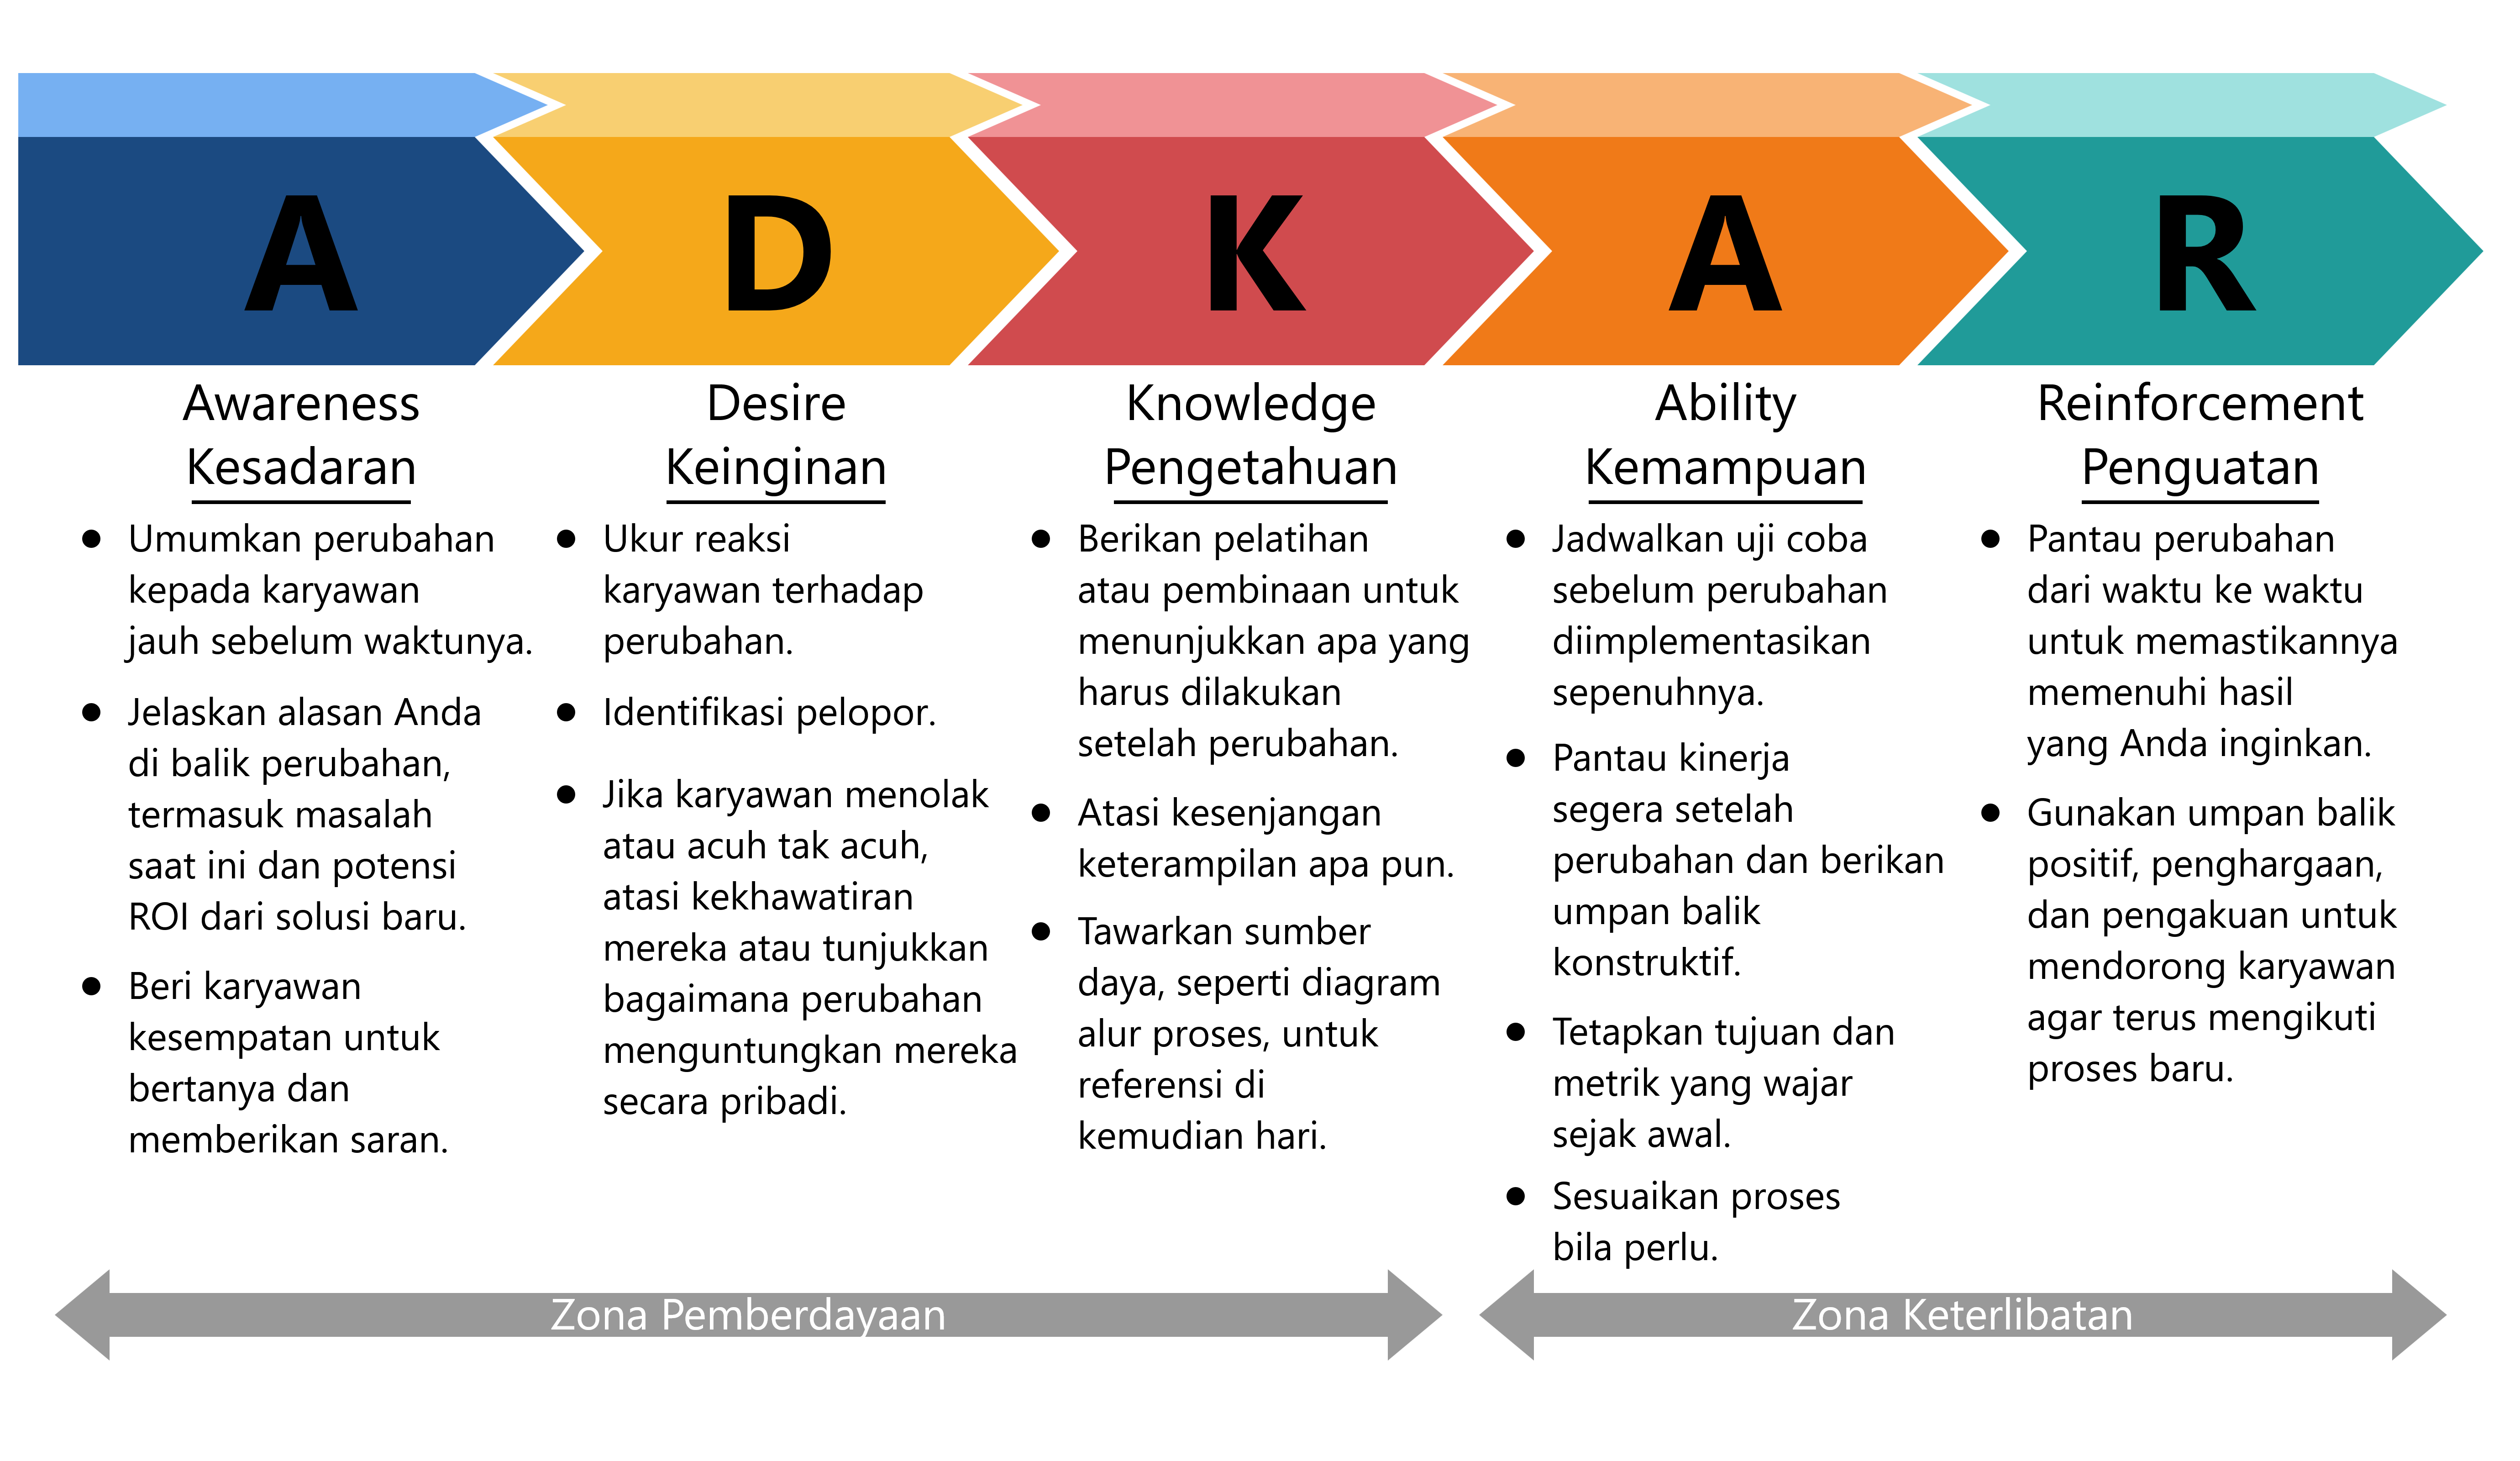
\includegraphics[width=0.98\linewidth,keepaspectratio]{assets/adkar.png}
        \end{tcolorbox}

        \column{0.45\textwidth}
        \begin{premiumbox}[Mitigasi 4 Pola Resistensi]
            \scriptsize
            ADKAR sebagai solusi terstruktur:
            \begin{itemize}
                \tiny
                \item \textbf{Kesadaran \& Keinginan:} Membangun urgensi \& kemauan untuk meninggalkan \textbf{Kebiasaan} lama dan menumbuhkan \textbf{Kepercayaan} pada sistem.
                \item \textbf{Pengetahuan \& Kemampuan:} Memberikan pembekalan teknis untuk menghilangkan celah \textbf{Kompetensi}.
                \item \textbf{Penguatan:} Memastikan keberlanjutan melalui kebijakan \textbf{Kewenangan} dan insentif KPI.
            \end{itemize}
        \end{premiumbox}
        \begin{orangebox}[Strategic Insight]
            \tiny Keberhasilan digitalisasi arsip di PLN ditentukan 20\% oleh teknologi dan 80\% oleh kesiapan manusia dalam mengadopsinya.
        \end{orangebox}
    \end{columns}
    \vfill
    \hfill{\fontsize{4}{5}\selectfont\color{gray}Ref: Hiatt, J. (2006). ADKAR: A Model for Change in Business, Government and our Community. Prosci.}\hspace{1em}
\end{frame}

% SLIDE 39: KOTTER'S 8-STEP MODEL
\begin{frame}{Leading Change: Kerangka Kerja Kotter (8-Step Model)}
    \begin{columns}
        \column{0.55\textwidth}
        \centering
        \begin{tcolorbox}[colback=white, colframe=plnblue!15, boxrule=0.5pt, arc=2pt, outer arc=2pt, left=2pt, right=2pt, top=2pt, bottom=2pt, boxsep=0pt, width=0.95\linewidth, drop shadow]
            \centering
            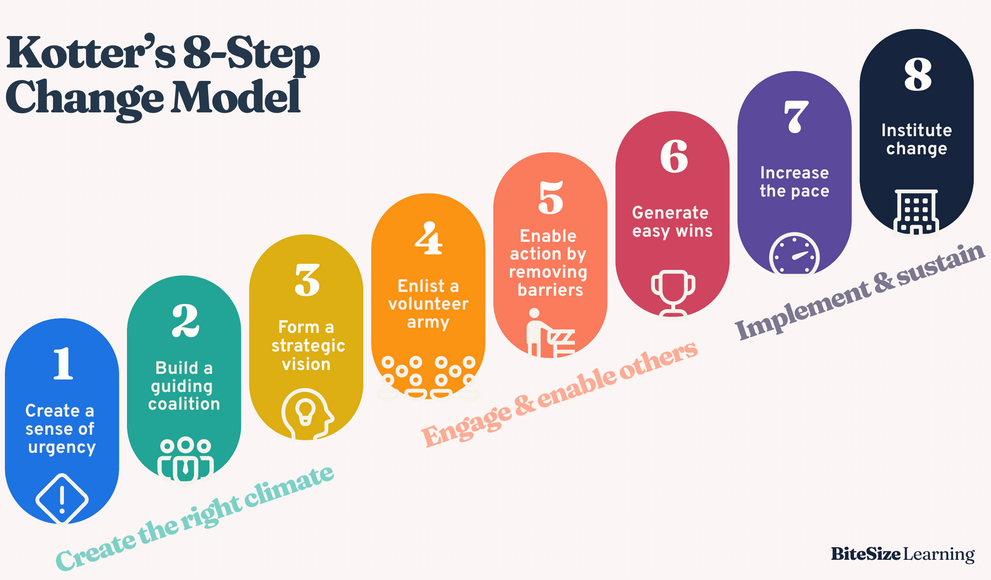
\includegraphics[width=0.9\linewidth,keepaspectratio]{assets/Kotters_8_Step.png}
        \end{tcolorbox}

        \column{0.45\textwidth}
        \begin{premiumbox}[Justifikasi 5 Strategi Mitigasi]
            \scriptsize
            Pendekatan PLN selaras dengan \textit{best practice} global:
            \begin{itemize}
                \tiny
                \item \textbf{Membentuk Koalisi:} Diimplementasikan melalui penunjukan \textbf{Duta Kearsipan} sebagai agen perubahan.
                \item \textbf{Capaian Jangka Pendek:} Dibuktikan melalui \textbf{Quick Win Pilot} di unit kerja prioritas.
                \item \textbf{Penguatan Budaya:} Pelembagaan perubahan melalui sistem \textbf{Insentif, Audit}, dan transparansi via \textbf{Dashboard}.
            \end{itemize}
        \end{premiumbox}
        \begin{greenbox}[Kematangan Organisasi]
            \tiny Transformasi digital yang sukses membutuhkan struktur kepemimpinan yang mampu mengawal perubahan dari tahap urgensi hingga menjadi budaya korporat baru.
        \end{greenbox}
    \end{columns}
    \vfill
    \hfill{\fontsize{4}{5}\selectfont\color{gray}Ref: Kotter, J.P. (1996). Leading Change. Harvard Business School Press.}\hspace{1em}
\end{frame}

% SLIDE 40: STAKEHOLDER MAP
\begin{frame}{Peta Pemangku Kepentingan \& Pendekatan}
    \vspace{0.2cm}
    \begin{table}
        \centering
        \tiny
        \begin{tabularx}{\textwidth}{@{} >{\raggedright\arraybackslash}X c >{\raggedright\arraybackslash}X >{\raggedright\arraybackslash}X @{}}
            \toprule
            \textbf{Pemangku Kepentingan} & \textbf{Peran} & \textbf{Motivasi} & \textbf{Pendekatan MA} \\
            \midrule
            General Manager/VP & Sponsor & Efisiensi biaya \& KPI & Laporan ROI berkala \\
            Manajer Area & Pemilik Proses & Kelancaran operasional & Wewenang pimpin \textit{pilot} \\
            Supervisor Senior & Pengamat Kritis & Stabilitas prosedur & Pendampingan personal \\
            Tim IT Fungsional & Mitra Teknis & Keamanan data & Koordinasi integrasi SLA \\
            Unit Kearsipan & Penjaga Standar & Kepatuhan ANRI & Validasi metadata \& JRA \\
            Auditor Internal & Penilai Kepatuhan & Transparansi & Akses dasbor audit trail \\
            \bottomrule
        \end{tabularx}
    \end{table}
    \vspace{0.2cm}
    \begin{greenbox}[Peringatan untuk Manajemen Atas]
        \scriptsize \textbf{Risiko terbesar} bukan kegagalan teknologi, melainkan \textbf{Shadow Systems}: personel tetap menjalankan prosedur manual secara diam-diam. Alokasikan minimal \textbf{30\% anggaran} untuk aktivitas manajemen perubahan.
    \end{greenbox}
\end{frame}

% SLIDE 41: POWER-INTEREST GRID
\begin{frame}{Analisis Matriks: Power vs Interest Grid}
    \begin{columns}
        \column{0.55\textwidth}
        \centering
        \begin{tcolorbox}[colback=white, colframe=plnblue!15, boxrule=0.5pt, arc=2pt, outer arc=2pt, left=2pt, right=2pt, top=2pt, bottom=2pt, boxsep=0pt, width=0.95\linewidth, drop shadow]
            \centering
            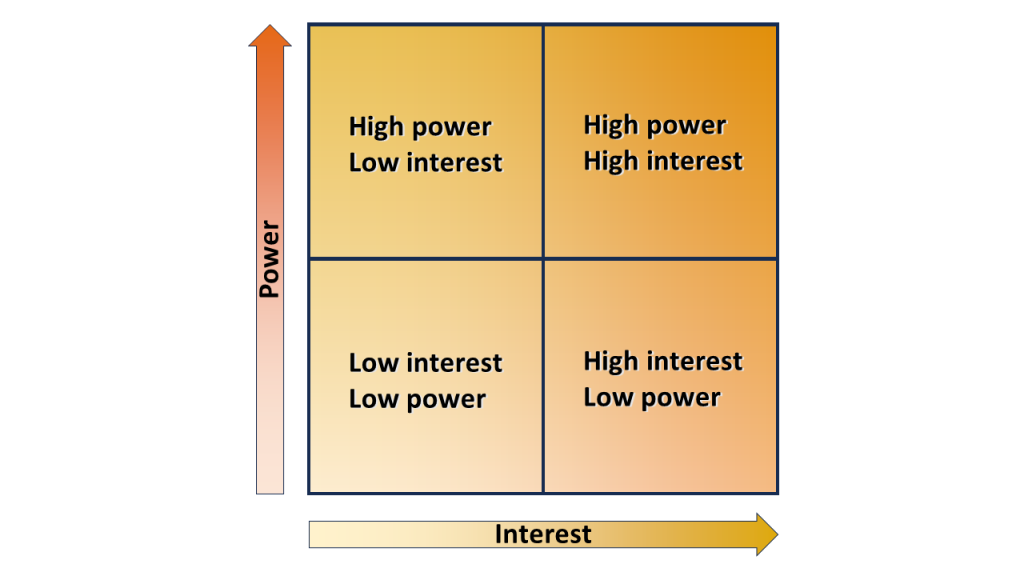
\includegraphics[width=0.9\linewidth,keepaspectratio]{assets/Power-Interest_Grid.png}
        \end{tcolorbox}

        \column{0.45\textwidth}
        \begin{premiumbox}[Klasifikasi Strategi Engagement]
            \scriptsize
            Pemetaan dari tabel pemangku kepentingan:
            \begin{itemize}
                \tiny
                \item \textbf{Kelola Secara Intensif (High P/H I):} General Manager, VP, \& Manajer Area (Fokus utama dukungan \& kendali).
                \item \textbf{Jaga Kepuasan (High P/L I):} Supervisor Senior \& Auditor (Butuh bukti kepatuhan \& efisiensi).
                \item \textbf{Tetap Berikan Informasi (Low P/H I):} Tim IT \& Unit Kearsipan (Mitra kolaborasi teknis operasional).
            \end{itemize}
        \end{premiumbox}
        \begin{orangebox}[Strategic Priority]
            \tiny Strategi komunikasi harus disesuaikan dengan posisi tiap kelompok di dalam matriks untuk meminimalkan friksi dan memaksimalkan adopsi.
        \end{orangebox}
    \end{columns}
    \vfill
    \hfill{\fontsize{4}{5}\selectfont\color{gray}Ref: Mendelow, A.L. (1991). ``Environmental Scanning: The Impact of the Stakeholder Concept''. ICIS Proceedings.}\hspace{1em}
\end{frame}

% SLIDE 42: ROADMAP & RENCANA AKSI
\begin{frame}{Rencana Aksi 30 Hari \& Budaya Kerja}
    \begin{columns}[T]
        \column{0.5\textwidth}
        \begin{premiumbox}[Target Capaian Mingguan]
            \scriptsize
            \begin{description}
                \item[\textbf{M1}] \textit{Pilot Launch:} Integrasi API \& pelatihan personel unit percontohan.
                \item[\textbf{M2}] \textit{Parallel Run:} Jalankan proses lama \& baru secara bersamaan.
                \item[\textbf{M3}] \textit{Cut-Off:} Hentikan proses lama, sediakan \textit{helpdesk}.
                \item[\textbf{M4}] \textit{Standardisasi:} Evaluasi KPI, publikasikan \textit{quick win}, standardisasi SOP.
            \end{description}
        \end{premiumbox}
        
        \column{0.5\textwidth}
        \begin{orangebox}[Program ``Duta Kearsipan'']
            \small Mendukung \textbf{Budaya Digital} di tiap unit melalui pelatihan dan pendampingan sebaya.
        \end{orangebox}
        \vspace{0.2cm}
        \begin{greenbox}[Kunci Sukses Implementasi]
            \scriptsize
            Jangan pernah mempermalukan personel yang lambat beradaptasi. Gunakan pendekatan \textit{``kita belajar bersama''} dan akui bahwa perubahan memerlukan waktu.
        \end{greenbox}
    \end{columns}
\end{frame}

% SLIDE 40: OUTPUT PORTOFOLIO
\begin{frame}{Rangkuman: 4 Dokumen Portofolio Wajib}
    \vspace{0.3cm}
    \begin{columns}[T]
        \column{0.24\textwidth}
        \centering
        \stepicon{plnblue}{1}\\[0.1cm]
        \textbf{Matriks Identifikasi Area Optimasi}\\[0.1cm]
        \tiny Kriteria 4.3.1\\[0.1cm]
        \scriptsize Pemetaan hambatan \& potensi integrasi (Bab 2).
        
        \column{0.24\textwidth}
        \centering
        \stepicon{plncyan}{2}\\[0.1cm]
        \textbf{Diagram BPMN 2.0 (To-Be)}\\[0.1cm]
        \tiny Kriteria 4.3.2\\[0.1cm]
        \scriptsize Alur kerja + Peta Pemicu Integrasi (Bab 3).
        
        \column{0.24\textwidth}
        \centering
        \stepicon{plnorange}{3}\\[0.1cm]
        \textbf{Draft SOP Digital Terintegrasi}\\[0.1cm]
        \tiny Kriteria 4.3.3\\[0.1cm]
        \scriptsize 8 Komponen wajib + metadata (Bab 4).
        
        \column{0.24\textwidth}
        \centering
        \stepicon{plngreen}{4}\\[0.1cm]
        \textbf{KPI Tracker + Business Case}\\[0.1cm]
        \tiny Kriteria 4.3.4\\[0.1cm]
        \scriptsize ROI + Rencana Aksi 30 Hari (Bab 5).
    \end{columns}
    \vspace{0.4cm}
    \begin{premiumbox}[Kriteria Kelulusan]
        \scriptsize
        \stepicon{plnblue}{\checkmark} 4 dokumen portofolio lengkap \quad
        \stepicon{plncyan}{\checkmark} Skor rubrik $\geq$ 70/100 \quad
        \stepicon{plnorange}{\checkmark} Post-test $\geq$ 65 \quad
        \stepicon{plngreen}{\checkmark} Komitmen tindak lanjut tertulis
    \end{premiumbox}
\end{frame}

% SLIDE 41: EXECUTIVE TOLLGATE (STRATEGIC CHECKLIST)
\begin{frame}{Executive Tollgate: Matriks Keputusan Strategis}
    \centering
    \begin{columns}
        \column{0.42\textwidth}
        \centering
        \begin{tikzpicture}[
            gate/.style={circle, draw=plnblue, fill=white, thick, minimum size=0.8cm, font=\bfseries},
            line/.style={ultra thick, plnblue!30}
        ]
            % Vertical Path
            \draw[line] (0, 3.4) -- (0, -0.6);
            
            % Tollgate nodes
            \node[gate, fill=plnblue!10] (g1) at (0, 3) {1};
            \node[gate, fill=plncyan!10, draw=plncyan] (g2) at (0, 1.8) {2};
            \node[gate, fill=plnorange!10, draw=plnorange] (g3) at (0, 0.6) {3};
            \node[gate, fill=plngreen!10, draw=plngreen] (g4) at (0, -0.6) {4};
            
            % Labels to the right
            \node[anchor=west, font=\scriptsize\bfseries] at (0.6, 3) {Legal Compliance Gate};
            \node[anchor=west, font=\scriptsize\bfseries] at (0.6, 1.8) {Data Integrity Gate};
            \node[anchor=west, font=\scriptsize\bfseries] at (0.6, 0.6) {Operational Value Gate};
            \node[anchor=west, font=\scriptsize\bfseries] at (0.6, -0.6) {Scalability Gate};
        \end{tikzpicture}
        
        \column{0.58\textwidth}
        \begin{premiumbox}[Kriteria Verifikasi Pimpinan]
            \tiny
            \begin{itemize}
                \item[\tikz{\node[draw=plnblue, fill=plnblue!10, inner sep=1pt, minimum size=0.3cm] {\tiny\checkmark};}] \textbf{G1: Legal} --- Apakah alur kerja selaras dengan tata naskah dinas \& ISO 15489?
                \item[\tikz{\node[draw=plnblue, fill=plnblue!10, inner sep=1pt, minimum size=0.3cm] {\tiny\checkmark};}] \textbf{G2: Integrity} --- Apakah \textit{audit trail} \& TTE sudah menjamin keaslian arsip?
                \item[\tikz{\node[draw=plnblue, fill=plnblue!10, inner sep=1pt, minimum size=0.3cm] {\tiny\checkmark};}] \textbf{G3: Value} --- Apakah potensi efisiensi (\textit{time/cost}) sudah tervalidasi?
                \item[\tikz{\node[draw=plnblue, fill=plnblue!10, inner sep=1pt, minimum size=0.3cm] {\tiny\checkmark};}] \textbf{G4: Scale} --- Apakah infrastruktur IT siap untuk volume data jangka panjang?
            \end{itemize}
        \end{premiumbox}
        
        \begin{orangebox}[Strategic Verdict]
            \scriptsize Jika salah satu gate bernilai \textbf{"No"}, segera lakukan re-evaluasi pada Bab Diagnosis atau Bab Desain SOP sebelum melanjutkan implementasi.
        \end{orangebox}
    \end{columns}
\end{frame}

% SLIDE 42: REFLEKSI & KOMITMEN (FIX #5)
\begin{frame}{Refleksi Pembelajaran \& Komitmen Tindak Lanjut}
    \vspace{0.2cm}
    \begin{premiumbox}[Pertanyaan Refleksi Mandiri]
        \small
        \begin{enumerate}
            \item Apa \textbf{1 proses kearsipan} yang paling mendesak untuk dioptimalkan di unit Anda?
            \item Siapa \textbf{pemangku kepentingan kunci} (IT, GCG, Operasional) yang perlu dilibatkan sejak awal?
            \item \textbf{Hambatan budaya} atau prosedur apa yang paling mungkin muncul, dan bagaimana mitigasinya?
        \end{enumerate}
    \end{premiumbox}
    \vspace{0.2cm}
    \begin{orangebox}[Lembar Komitmen 30 Hari]
        \small
        Saya, \underline{\hspace{3.5cm}}, menyatakan akan menginisiasi pilot optimalisasi alur kerja pada proses \underline{\hspace{3.5cm}} dengan target KPI \underline{\hspace{2.5cm}} dan melaporkan hasil monitoring kepada \underline{\hspace{3cm}} paling lambat tanggal~\underline{\hspace{2.5cm}}.
    \end{orangebox}
\end{frame}

% SLIDE 42: CLOSING (FIX #10: Penutup Bermakna)
\begin{frame}{}
    \vspace{0.5cm}
    \begin{center}
        \huge \textcolor{plnblue}{\textbf{TERIMA KASIH}}\\[0.3cm]
        \large Mari Menuju Ekosistem Informasi yang Adaptif dan Otentik!\\[0.6cm]
        \normalsize \textit{``Optimalisasi hari ini untuk Keandalan hari esok.''}
    \end{center}
    \vspace{0.4cm}
    \begin{center}
        \begin{minipage}{0.65\textwidth}
            \begin{greenbox}[Langkah Selanjutnya]
                \scriptsize
                \begin{itemize}
                    \item Kerjakan \textbf{Post-Test} (10 soal)
                    \item Kumpulkan \textbf{4 portofolio} ke Unit Kearsipan
                    \item Jadwalkan \textbf{Peer Review Session} antar unit
                    \item Gunakan modul sebagai acuan \textbf{Rencana Peningkatan Tahunan}
                \end{itemize}
            \end{greenbox}
        \end{minipage}
    \end{center}
\end{frame}

\end{document}
